
%%%%%%%%%%%%%%%%%%%%%%%%%%%%%%%%%%%%%%%%%
% Short Sectioned Assignment LaTeX Template Version 1.0 (5/5/12)
% This template has been downloaded from: http://www.LaTeXTemplates.com
% Original author:  Frits Wenneker (http://www.howtotex.com)
% License: CC BY-NC-SA 3.0 (http://creativecommons.org/licenses/by-nc-sa/3.0/)
%%%%%%%%%%%%%%%%%%%%%%%%%%%%%%%%%%%%%%%%%

%----------------------------------------------------------------------------------------
%	PACKAGES AND OTHER DOCUMENT CONFIGURATIONS
%----------------------------------------------------------------------------------------

\documentclass[paper=a4, fontsize=11pt]{scrartcl} % A4 paper and 11pt font size

% ---- Entrada y salida de texto -----

\usepackage[T1]{fontenc} % Use 8-bit encoding that has 256 glyphs
\usepackage[utf8]{inputenc}
%\usepackage{fourier} % Use the Adobe Utopia font for the document - comment this line to return to the LaTeX default

% ---- Idioma --------

\usepackage[spanish, es-tabla]{babel} % Selecciona el español para palabras introducidas automáticamente, p.ej. "septiembre" en la fecha y especifica que se use la palabra Tabla en vez de Cuadro

% ---- Otros paquetes ----

\usepackage{url} % ,href} %para incluir URLs e hipervínculos dentro del texto (aunque hay que instalar href)
\usepackage{amsmath,amsfonts,amsthm} % Math packages
%\usepackage{graphics,graphicx, floatrow} %para incluir imágenes y notas en las imágenes
\usepackage{graphics,graphicx, float} %para incluir imágenes y colocarlas
\usepackage{movie15}

% Para hacer tablas comlejas
%\usepackage{multirow}
%\usepackage{threeparttable}

%\usepackage{sectsty} % Allows customizing section commands
%\allsectionsfont{\centering \normalfont\scshape} % Make all sections centered, the default font and small caps

\usepackage{fancyhdr} % Custom headers and footers

\pagestyle{fancyplain} % Makes all pages in the document conform to the custom headers and footers
\fancyhead{} % No page header - if you want one, create it in the same way as the footers below
\fancyfoot[L]{} % Empty left footer
\fancyfoot[C]{} % Empty center footer
\fancyfoot[R]{\thepage} % Page numbering for right footer
\renewcommand{\headrulewidth}{0pt} % Remove header underlines
\renewcommand{\footrulewidth}{0pt} % Remove footer underlines
\setlength{\headheight}{13.6pt} % Customize the height of the header

\numberwithin{equation}{section} % Number equations within sections (i.e. 1.1, 1.2, 2.1, 2.2 instead of 1, 2, 3, 4)
\numberwithin{figure}{section} % Number figures within sections (i.e. 1.1, 1.2, 2.1, 2.2 instead of 1, 2, 3, 4)
\numberwithin{table}{section} % Number tables within sections (i.e. 1.1, 1.2, 2.1, 2.2 instead of 1, 2, 3, 4)

\setlength\parindent{0pt} % Removes all indentation from paragraphs - comment this line for an assignment with lots of text

\newcommand{\horrule}[1]{\rule{\linewidth}{#1}} % Create horizontal rule command with 1 argument of height
\usepackage[breaklinks=true]{hyperref}
\usepackage{bookmark}
\usepackage{wasysym}
\usepackage{subcaption}
\usepackage[dvipsnames]{xcolor}
\usepackage{amssymb}
\usepackage{color}
\usepackage{listings}
\usepackage{upgreek} % para poner letras griegas sin cursiva
\usepackage{cancel} % para tachar
\usepackage{mathdots} % para el comando \iddots
\usepackage{mathrsfs} % para formato de letra
\usepackage{stackrel} % para el comando \stackbin
\lstdefinestyle{cmas}
{ %
	language=C++,                % elegir el lenguaje del código
	stringstyle=\color{blue}\ttfamily,,
	basicstyle=\normalsize\ttfamily,       % el tamaño del font a usar para el código
	numbers=left,                   % dónde poner los números de línea 
	numberstyle=\footnotesize,      % tamaño de font usados para los números de línea 
	stepnumber=1,                   % el paso de numeración
	numbersep=8pt,                  % distancia del numero de línea y la línea
	backgroundcolor=\color{white},  % color de fondo, para usarlo hay que agregar  \usepackage{color}
	showspaces=false,               % mostrar espacios en blanco ?
	showstringspaces=false,         % subrayar espacios con cadenas?   
	 showtabs=false,                 % mostrar taba usando cadenas? 
	frame=single,           			% enmarcar el código?  
	tabsize=2,          				% sets default tabsize to 2 spaces?
	keywordstyle=\color{MidnightBlue}\ttfamily\bfseries,
	commentstyle=\color{OliveGreen}\ttfamily,
	morecomment=[l][\color{OliveGreen}]{\#},
	captionpos=b,           % sets the caption-position to bottom?
	breaklines=true,        % sets automatic line breaking?
	breakatwhitespace=false,    % sets if automatic breaks should only happen at whitespace ?
	title=\lstname,
	escapeinside={\%*}{*)}          % if you want to add a comment within your code
}

\lstdefinestyle{payt}
{ %
	language=Python,                % elegir el lenguaje del código
	stringstyle=\color{blue}\ttfamily,,
	basicstyle=\normalsize\ttfamily,       % el tamaño del font a usar para el código
	numbers=left,                   % dónde poner los números de línea 
	numberstyle=\footnotesize,      % tamaño de font usados para los números de línea 
	stepnumber=1,                   % el paso de numeración
	numbersep=8pt,                  % distancia del numero de línea y la línea
	backgroundcolor=\color{white},  % color de fondo, para usarlo hay que agregar  \usepackage{color}
	showspaces=false,               % mostrar espacios en blanco ?
	showstringspaces=false,         % subrayar espacios con cadenas?   
	showtabs=false,                 % mostrar taba usando cadenas? 
	frame=single,           			% enmarcar el código?  
	tabsize=2,          				% sets default tabsize to 2 spaces?
	keywordstyle=\color{MidnightBlue}\ttfamily\bfseries,
	commentstyle=\color{OliveGreen}\ttfamily,
	morecomment=[l][\color{OliveGreen}]{\#},
	captionpos=b,           % sets the caption-position to bottom?
	breaklines=true,        % sets automatic line breaking?
	breakatwhitespace=false,    % sets if automatic breaks should only happen at whitespace ?
	title=\lstname,
	escapeinside={\%*}{*)}          % if you want to add a comment within your code
}

\definecolor{light-gray}{gray}{0.85}

\lstdefinestyle{fich}
{ %
	language=Bash,                % elegir el lenguaje del código
	stringstyle=\color{black}\texttt,
	basicstyle=\normalsize\ttfamily,       % el tamaño del font a usar para el código	
	numbers=left,                   % dónde poner los números de línea 
	numberstyle=\footnotesize,      % tamaño de font usados para los números de línea 
	stepnumber=1,                   % el paso de numeración
	numbersep=8pt,                  % distancia del numero de línea y la línea
	backgroundcolor=\color{light-gray},  % color de fondo, para usarlo hay que agregar  \usepackage{color}
	showspaces=false,               % mostrar espacios en blanco ?
	showstringspaces=false,         % subrayar espacios con cadenas?   
	showtabs=false,                 % mostrar taba usando cadenas? 
%	frame=single,           			% enmarcar el código?  
	tabsize=2,          				% sets default tabsize to 2 spaces?
	captionpos=b,           % sets the caption-position to bottom?
	breaklines=true,        % sets automatic line breaking?
	breakatwhitespace=false,    % sets if automatic breaks should only happen at whitespace ?
	title=\lstname,
	escapeinside={\%*}{*)}          % if you want to add a comment within your code
}

\lstset{literate=
  {á}{{\'a}}1 {é}{{\'e}}1 {í}{{\'i}}1 {ó}{{\'o}}1 {ú}{{\'u}}1
  {Á}{{\'A}}1 {É}{{\'E}}1 {Í}{{\'I}}1 {Ó}{{\'O}}1 {Ú}{{\'U}}1
  {à}{{\`a}}1 {è}{{\`e}}1 {ì}{{\`i}}1 {ò}{{\`o}}1 {ù}{{\`u}}1
  {À}{{\`A}}1 {È}{{\'E}}1 {Ì}{{\`I}}1 {Ò}{{\`O}}1 {Ù}{{\`U}}1
  {ä}{{\"a}}1 {ë}{{\"e}}1 {ï}{{\"i}}1 {ö}{{\"o}}1 {ü}{{\"u}}1
  {Ä}{{\"A}}1 {Ë}{{\"E}}1 {Ï}{{\"I}}1 {Ö}{{\"O}}1 {Ü}{{\"U}}1
  {â}{{\^a}}1 {ê}{{\^e}}1 {î}{{\^i}}1 {ô}{{\^o}}1 {û}{{\^u}}1
  {Â}{{\^A}}1 {Ê}{{\^E}}1 {Î}{{\^I}}1 {Ô}{{\^O}}1 {Û}{{\^U}}1
  {œ}{{\oe}}1 {Œ}{{\OE}}1 {æ}{{\ae}}1 {Æ}{{\AE}}1 {ß}{{\ss}}1
  {ű}{{\H{u}}}1 {Ű}{{\H{U}}}1 {ő}{{\H{o}}}1 {Ő}{{\H{O}}}1
  {ç}{{\c c}}1 {Ç}{{\c C}}1 {ø}{{\o}}1 {å}{{\r a}}1 {Å}{{\r A}}1
  {€}{{\EUR}}1 {£}{{\pounds}}1
  {ñ}{{\~n}}1
}

\hypersetup{
    colorlinks=true,
    linkcolor=black,
    filecolor=magenta,      
    urlcolor=blue,
    pdftitle={ISE: Práctica 3 - Mario Rodríguez Ruiz},
    bookmarks=true,
    citecolor=blue,
}



%----------------------------------------------------------------------------------------
%	TÍTULO Y DATOS DEL ALUMNO
%----------------------------------------------------------------------------------------

\title{	
\normalfont \normalsize 
\textsc{\textbf{Ingeniería de Servidores (2016-2017)} \\ Subgrupo A1 \\ Grado en Ingeniería Informática\\ Universidad de Granada} \\ [25pt] % Your university, school and/or department name(s)
\horrule{0.5pt} \\[0.4cm] % Thin top horizontal rule
\huge Práctica 2: Instalación y configuración de servicios \\ % The assignment title
\horrule{2pt} \\[0.5cm] % Thick bottom horizontal rule
}

\author{Mario Rodríguez Ruiz} % Nombre y apellidos

\date{\normalsize\today} % Incluye la fecha actual

%----------------------------------------------------------------------------------------
% DOCUMENTO
%----------------------------------------------------------------------------------------

\begin{document}

\maketitle % Muestra el Título

\newpage %inserta un salto de página

\tableofcontents % para generar el índice de contenidos

\listoffigures

\newpage

%----------------------------------------------------------------------------------------
%	Cuestión 1
%----------------------------------------------------------------------------------------

\section{Cuestión 1}
\subsection{Liste los argumentos de yum necesarios para instalar,
	buscar y eliminar paquetes}

Argumentos de \textbf{yum}\cite{enlace5}:
\begin{itemize}
	\item Para instalar: \textbf{$ > $ sudo yum install \textit{paquete}}
	
	En la Figura \ref{fig:figura1} se muestra la instalación el paquete \textbf{epel-release} desde Centos 7.
	\begin{figure}[H] %con el [H] le obligamos a situar aquí la figura
		\centering
		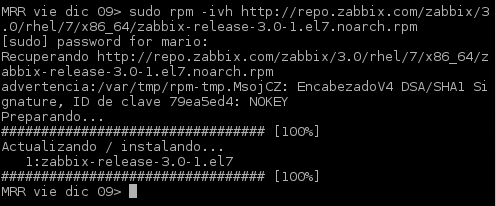
\includegraphics[scale=0.7]{figuras/figura1.png} 
		\caption{Instalación del paquete \textbf{epel-release}} 
		\label{fig:figura1}
	\end{figure}
	
	\item Para buscar: \textbf{$ > $ yum search \textit{paquete}}
	
	En la Figura \ref{fig:figura3} se muestra la búsqueda del paquete \textbf{kernel-devel} desde Centos 7.
	\begin{figure}[H] %con el [H] le obligamos a situar aquí la figura
		\centering
		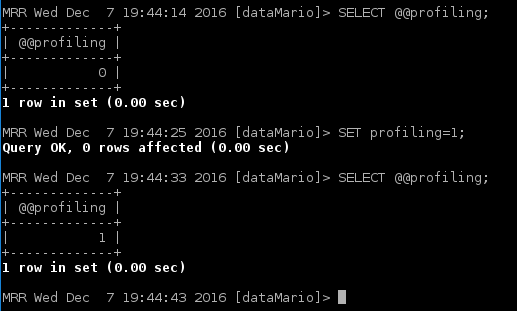
\includegraphics[scale=0.7]{figuras/figura3.png} 
		\caption{Búsqueda del paquete \textbf{kernel-devel}} 
		\label{fig:figura3}
	\end{figure}

\newpage
	
	\item Para borrar: \textbf{$ > $ sudo yum remove \textit{paquete}}
	
	En la Figura \ref{fig:figura2} se muestra cómo se borra el paquete \textbf{kernel-headers} desde Centos 7.
	\begin{figure}[H] %con el [H] le obligamos a situar aquí la figura
		\centering
		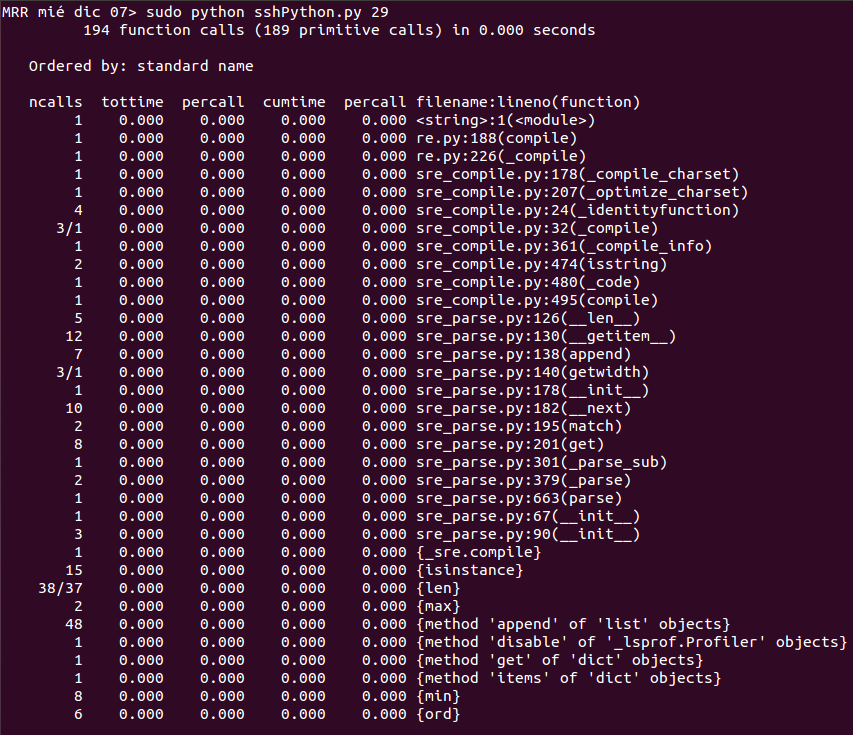
\includegraphics[scale=0.7]{figuras/figura2.png} 
		\caption{Borrado del paquete \textbf{kernel-headers}} 
		\label{fig:figura2}
	\end{figure}			
\end{itemize}
\subsection{¿Qué ha de hacer para que yum pueda tener
	acceso a Internet en el PC del aula?(Pistas: archivo de configuración en /etc,	proxy: stargate.ugr.es:3128)}

Para que \textbf{yum} pueda tener acceso a Internet en el PC del aula hay que editar el fichero de configuración \textbf{/etc/yum.conf}\cite{enlace3} añadiéndole una nueva linea que contendrá lo siguiente: 

\begin{center}
	\textbf{proxy=stargate.ugr.es:3128}
\end{center}

\subsection{¿Cómo añadimos un nuevo repositorio?}

Para añadir un nuevo repositorio se utiliza la herramienta \textbf{yum-config-manager}\cite{enlace4} que permite, entre otras, dicha gestión. Un ejemplo de ejecución sería:

\begin{center}
	$ > $ \textbf{yum-config-manager –add-repo=url}
\end{center}

En la Figura \ref{fig:figura4} se muestra cómo se añade el repositorio \textbf{kde.repo} desde Centos 7.

\begin{figure}[H] %con el [H] le obligamos a situar aquí la figura
	\centering
	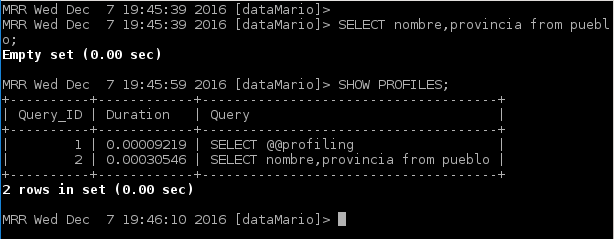
\includegraphics[scale=0.7]{figuras/figura4.png} 
	\caption{Añadido del repositorio \textbf{kde.repo}} 
	\label{fig:figura4}
\end{figure}

\newpage

%----------------------------------------------------------------------------------------
%	Cuestión 2
%----------------------------------------------------------------------------------------

\section{Cuestión 2}
\subsection{Liste los argumentos de apt necesarios para instalar, buscar
	y eliminar paquetes.}

Argumentos de \textbf{apt}\cite{enlace6}:
\begin{itemize}
	\item Para instalar: \textbf{$ > $ sudo apt-get install \textit{paquete}}\cite{enlace6}
	
	En la Figura \ref{fig:figura5} se muestra cómo se instala el paquete \textbf{gcc} en Ubuntu Server.
	\begin{figure}[H] %con el [H] le obligamos a situar aquí la figura
		\centering
		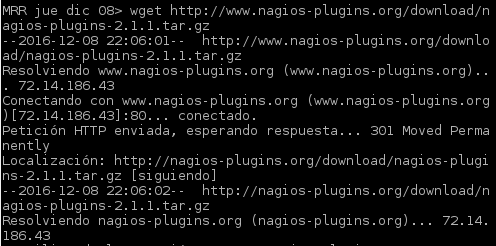
\includegraphics[scale=0.6]{figuras/figura5.png} 
		\caption{Instalación del paquete \textbf{gcc}} 
		\label{fig:figura5}
	\end{figure}
	
	\item Para buscar: \textbf{$ > $ apt-cache search \textit{paquete}}\cite{enlace6}
	
	En la Figura \ref{fig:figura6} se muestra cómo se busca el paquete \textbf{gedit} en Ubuntu Server.
	\begin{figure}[H] %con el [H] le obligamos a situar aquí la figura
		\centering
		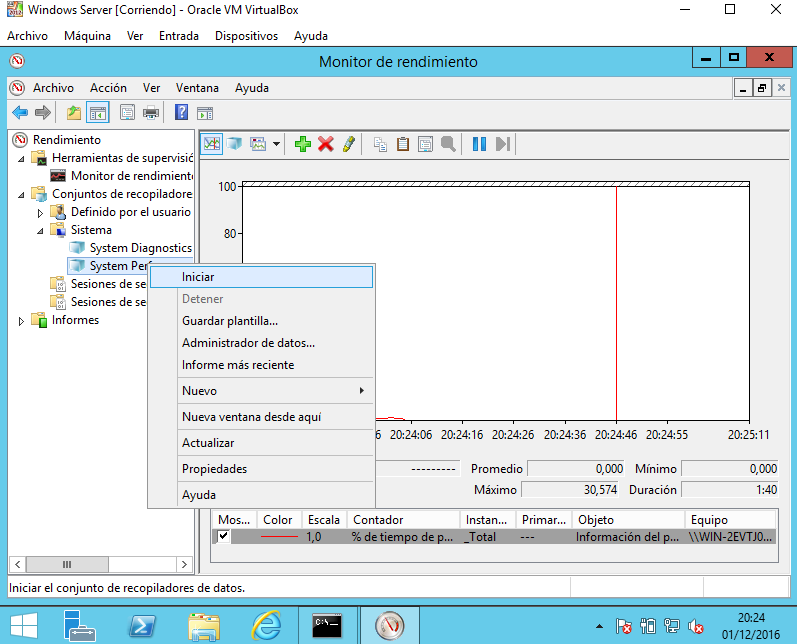
\includegraphics[scale=0.8]{figuras/figura6.png} 
		\caption{Búsqueda del paquete \textbf{gedit}} 
		\label{fig:figura6}
	\end{figure}

\newpage

	\item Para borrar: \textbf{$ > $ sudo apt remove \textit{paquete}}\cite{enlace6}
	
	En la Figura \ref{fig:figura7} se muestra cómo se borra el paquete \textbf{gedit} en Ubuntu Server.
	\begin{figure}[H] %con el [H] le obligamos a situar aquí la figura
		\centering
		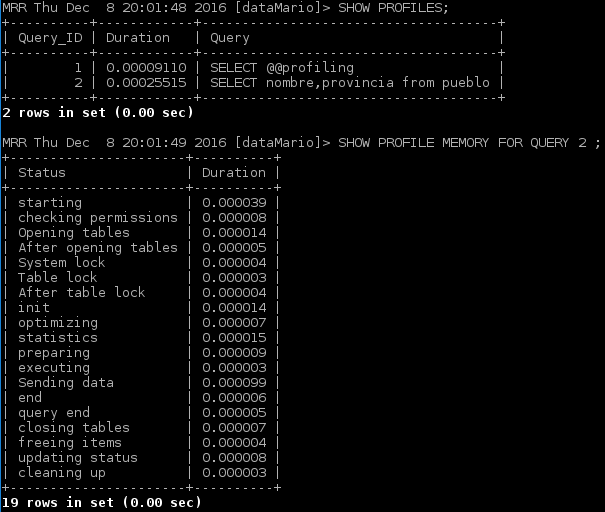
\includegraphics[scale=0.6]{figuras/figura7.png} 
		\caption{Borrado del paquete \textbf{gedit}} 
		\label{fig:figura7}
	\end{figure}			
\end{itemize}

\subsection{¿Qué ha de hacer para que apt pueda tener acceso a
	Internet en el PC del aula?(Pistas: archivo de configuración en /etc, proxy:stargate.ugr.es:3128)}

Para que \textbf{apt} pueda tener acceso a Internet en el PC del aula existen tres métodos\cite{enlace8}:

\begin{itemize}
	\item Sesión de proxy temporal.
	
	Este modo de acceso se debe configurar manualmente cada vez que desee utilizar apt-get a través de un proxy HTTP. 
	
	Para ello se debe de introducir la siguiente orden en un terminal:	
	\begin{center}
		\textbf{$ > $ export http\_proxy  =  http:  $ // $  stargate.ugr.es: 3128 }
	\end{center}

	\item Modificación del fichero de configuración de APT.
	
	Editar el fichero de configuración \textbf{/etc/apt.conf}\cite{enlace7} añadiéndole una nueva linea que contendrá lo siguiente: 
	
	\begin{center}
		\textbf{Acquire :: http :: Proxy $ " $http: $ // $ stargate.ugr.es: 3128$ " $ ;}
	\end{center}

	\item Modificación del fichero de configuración de BASH\cite{enlace9}.
	
	Editar el fichero de configuración  \textbf{ \AC $ /. $bashrc} añadiéndole dos nuevas lineas que contendrán lo siguiente: 
	
	
	\textbf{http\_proxy = http: $ // $ stargate.ugr.es: 3128}
	
	\textbf{export http\_proxy}
	
	
\end{itemize}

\subsection{¿Cómo añadimos un nuevo repositorio?}

Para añadir un nuevo repositorio se introduce la siguiente orden en un terminal\cite{enlace10,enlace11}: 

\begin{center}
	\textbf{$ > $ sudo add-apt-repository ppa:\textit{repositorio}}
\end{center}

Donde \textit{repositorio} es el nombre del repositorio a añadir.
\begin{figure}[H] %con el [H] le obligamos a situar aquí la figura
	\centering
	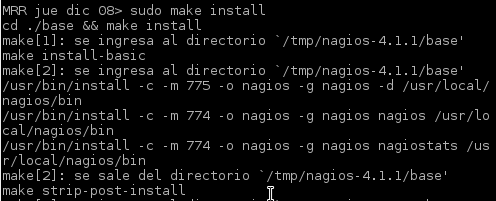
\includegraphics[scale=0.7]{figuras/figura8.png} 
	\caption{Añadido del repositorio \textbf{shutter}} 
	\label{fig:figura8}
\end{figure}

En la Figura \ref{fig:figura8} se muestra cómo se añade el repositorio \textbf{shutter} en Ubuntu Server.

\newpage

%----------------------------------------------------------------------------------------
%	Cuestión 3
%----------------------------------------------------------------------------------------

\section{Cuestión 3}
\subsection{¿Con qué comando puede abrir/cerrar un puerto usando
	ufw? Muestre un ejemplo de cómo lo ha hecho}

Comandos \textbf{ufw}\cite{enlace12}:
\begin{itemize}
	\item Para abrir un puerto: \textbf{$ > $ sudo ufw allow \textit{puerto}}\cite{enlace12}
	
	Al no tener activo el servicio, primero hay que activarlo y luego establecerle
	una configuración determinada: En este caso se ha denegado cualquier conexión entrante con la especificación \textbf{default deny}.
	
	A continuación se reinicia el servicio, desactivándolo y activándolo de forma seguida.
	
	Por último se abre el puerto 22.
	\\
	
	En la Figura \ref{fig:figura9} se muestra todo el proceso descrito anteriormente.
	\begin{figure}[H] %con el [H] le obligamos a situar aquí la figura
		\centering
		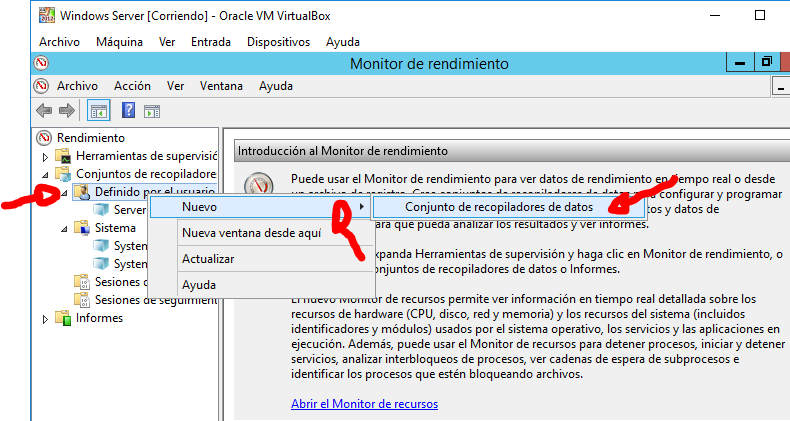
\includegraphics[scale=0.8]{figuras/figura9.png} 
		\caption{Apertura del puerto \textbf{22} (SSH) con ufw} 
		\label{fig:figura9}
	\end{figure}
		
	\item Para cerrar un puerto: \textbf{$ > $ sudo ufw deny \textit{puerto}}\cite{enlace12}
	
	En la Figura \ref{fig:figura10} se muestra en primer lugar el estado actual de los puertos. Aparece el como abierto el puerto 22, por lo que se procede a cerrarlo.
	
	
	De nuevo se comprueba el estado de los puertos y se aprecia cómo ya esta cerrado.
	\begin{figure}[H] %con el [H] le obligamos a situar aquí la figura
		\centering
		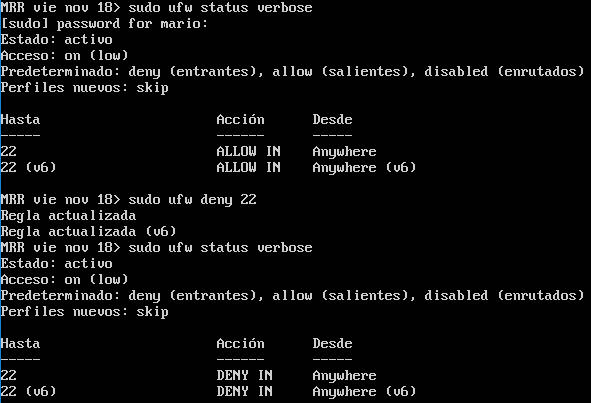
\includegraphics[scale=0.8]{figuras/figura10.png} 
		\caption{Denegado el acceso a través del puerto \textbf{22} (SSH) con ufw} 
		\label{fig:figura10}
	\end{figure}				
\end{itemize}

\subsection{¿Con qué comando puede
	abrir/cerrar un puerto usando firewall-cmd en CentOS? Muestre un ejemplo
	de cómo lo ha hecho}

Comandos \textbf{firewall-cmd}:
\begin{itemize}
	\item Para abrir un puerto: \textbf{$ > $ firewall-cmd --zone=\textit{zona} --add-port=\textit{puerto}/\textit{protocolo}}\cite{enlace13,enlace14}
	
	En la Figura \ref{fig:figura11} se muestra en primer lugar el la lista actual de los puertos abiertos. De forma seguida se abre el puerto 22/tcp.
	\begin{figure}[H] %con el [H] le obligamos a situar aquí la figura
		\centering
		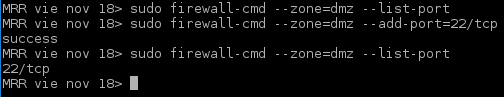
\includegraphics[scale=0.8]{figuras/figura11.png} 
		\caption{Apertura del puerto \textbf{22} (SSH) con firewall-cmd} 
		\label{fig:figura11}
	\end{figure}
	
	\item Para cerrar un puerto: \textbf{$ > $ firewall-cmd --zone=\textit{zona} --remove-port=\textit{puerto}/\textit{protocolo}}\cite{enlace13,enlace14}
	
	En la Figura \ref{fig:figura12} se muestra en primer lugar el la lista actual de los puertos abiertos. De forma seguida se abre el puerto 22/tcp.
	\begin{figure}[H] %con el [H] le obligamos a situar aquí la figura
		\centering
		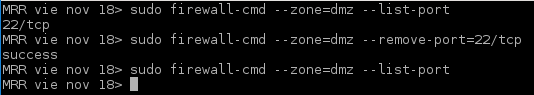
\includegraphics[scale=0.9]{figuras/figura12.png} 
		\caption{Denegado el acceso a través del puerto \textbf{22} (SSH) con firewall-cmd} 
		\label{fig:figura12}
	\end{figure}				
\end{itemize}

\subsection{Utilice el comando nmap para ver que,
	efectivamente, los puertos están accesibles} 

En la Figura \ref{fig:figura13} pueden verse los puertos que están accesibles mediante el comando \textbf{nmap} \cite{enlace15}. En primer lugar se muestran los accesibles desde el localhost y, en segundo lugar, los accesibles de una cualquier dirección al azar.

\begin{figure}[H] %con el [H] le obligamos a situar aquí la figura
	\centering
	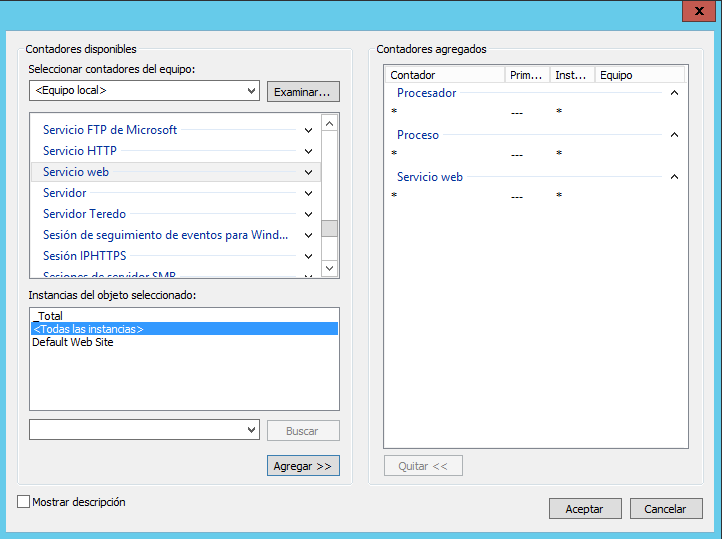
\includegraphics[scale=0.9]{figuras/figura13.png} 
	\caption{Muestra de los puertos accesibles con \textbf{nmap}} 
	\label{fig:figura13}
\end{figure}

\newpage


%----------------------------------------------------------------------------------------
%	Cuestión 4
%----------------------------------------------------------------------------------------

\section{Cuestión 4}
\subsection{¿Qué diferencia hay entre telnet y ssh?}

La diferencia más contundente que existe entre telnet y ssh es que \textbf{en ssh el tráfico se encuentra cifrado} y en telnet no.
Esto es por el uso que realiza SSH con claves criptográficas publicas y privadas. El par de claves SSH son generadas con algoritmos como RSA y DSA aunque ECDSA es el que recomienda  OpenSSH por ofrecer la misma seguridad con un menor tamaño en bits para las claves. 
\\

Otras diferencias son, por ejemplo, que funcionan en puertos diferentes: \textbf{telnet utiliza el puerto 23} mientras que ssh el 22 y que telnet usa un poco menos de sobrecarga de ancho de banda en comparación con ssh.
 

\cite{enlace1,enlace2}

%----------------------------------------------------------------------------------------
%	Cuestión 5
%----------------------------------------------------------------------------------------

\section{Cuestión 5}
\subsection{¿Para qué sirve la opción -X?}

La opción -X \cite{enlace16} sirve para habilitar el \textbf{X11 forwarding}. Éste permite que la aplicación gráfica se ejecute en el servidor y se exporte el display a la maquina cliente. Es decir, la aplicación simulará ejecutarse en la máquina anfitriona pero en realidad se estará ejecutando en el servidor.

\subsection{Ejecute remotamente, es
	decir, desde la máquina anfitriona (si tiene Linux) o desde la otra máquina
	virtual, el comando gedit en una sesión abierta con ssh. ¿Qué ocurre?}

En primer lugar se va a realizar una conexión desde la máquina de Ubuntu a la de Centos.

En la Figura \ref{fig:figura15} se muestra cuál es la dirección de la máquina de Centos para poder conectarse con ella.

\begin{figure}[H] %con el [H] le obligamos a situar aquí la figura
	\centering
	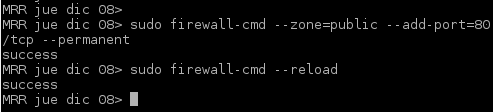
\includegraphics[scale=0.8]{figuras/figura15.png} 
	\caption{Muestra información de las interfaces de la máquina de CentOS} 
	\label{fig:figura15}
\end{figure}

La Figura \ref{fig:figura14} muestra la conexión entre las máquinas y, además, cómo no es posible la apertura gráfica de gedit, ya que este sistema operativo no dispone de interfaz gráfica de ventanas.

\begin{figure}[H] %con el [H] le obligamos a situar aquí la figura
	\centering
	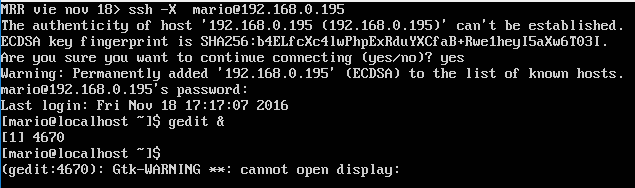
\includegraphics[scale=0.7]{figuras/figura14.png} 
	\caption{Ejecución remota de gedit desde la máquina Ubuntu S.} 
	\label{fig:figura14}
\end{figure}


Sin embargo, si la conexión se realiza de manera inversa (desde Ubuntu hacia Centos y siempre utilizando la opción -X en estos casos), no existe ningún problema. Véase en las Figuras \ref{fig:figura16} y \ref{fig:figura17} en las que se prueba dicha ejecución.

\begin{figure}[H] %con el [H] le obligamos a situar aquí la figura
	\centering
	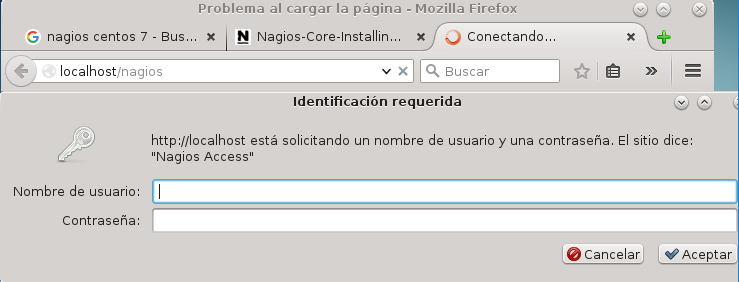
\includegraphics[scale=0.7]{figuras/figura16.png} 
	\caption{Muestra información de las interfaces de la máquina de Ubuntu S.} 
	\label{fig:figura16}
\end{figure}

La Figura \ref{fig:figura16} muestra la dirección de la máquina Ubuntu para poder realizar la conexión sobre ella.

\begin{figure}[H] %con el [H] le obligamos a situar aquí la figura
	\centering
	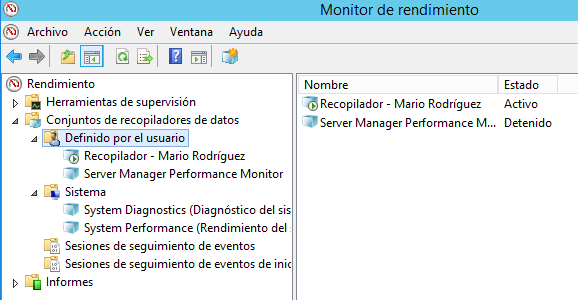
\includegraphics[scale=0.6]{figuras/figura17.png} 
	\caption{Ejecución remota de gedit desde la máquina CentOS} 
	\label{fig:figura17}
\end{figure}

Como se ve en la Figura \ref{fig:figura17} gedit no se encuentra instalado en la máquina CentOS,
por lo que se prueba que la ejecución se realiza en la máquina Ubuntu S..

\newpage

%----------------------------------------------------------------------------------------
%	Cuestión 6
%----------------------------------------------------------------------------------------
\section{Cuestión 6}
\subsection{Muestre la secuencia de comandos y las modificaciones a los
		archivos correspondientes para permitir acceder a la consola remota sin
		introducir la contraseña. Pruebe que funciona. (Pistas: ssh-keygen, ssh-copyid).}
	
En primer lugar se generan las claves RSA en el host desde el que va a realizar la conexión (CentOS, en este caso) a través del comando:

\textbf{$ > $ ssh-keygen -t rsa} \cite{enlace17}
\\

La Figura \ref{fig:figura97} muestra la creación de las claves ECDSA para su posterior utilización en SSH.

\begin{figure}[H] %con el [H] le obligamos a situar aquí la figura
	\centering
	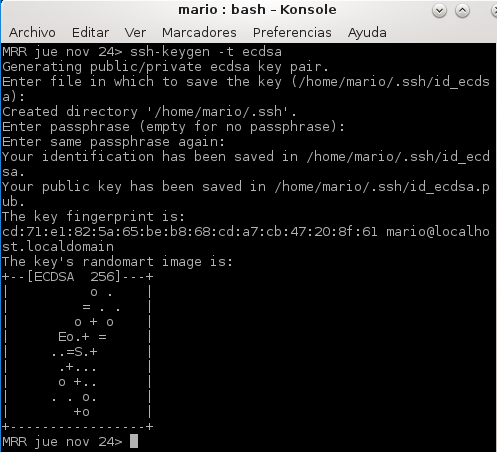
\includegraphics[scale=0.8]{figuras/figura97.png} 
	\caption{Creación de las claves RSA} 
	\label{fig:figura97}
\end{figure}

A continuación, desde el mismo host (CentOS), se copiará la clave generada anteriormente
en el host al que se quiere conectar (Ubuntu S.) por medio de la orden \cite{enlace18}:

\textbf{$ > $ ssh-copy-id \textit{usuario}@\textit{ip}}

\newpage

La Figura \ref{fig:figura98} muestra cómo se copian las claves en el host destino a través de su IP.

\begin{figure}[H] %con el [H] le obligamos a situar aquí la figura
	\centering
	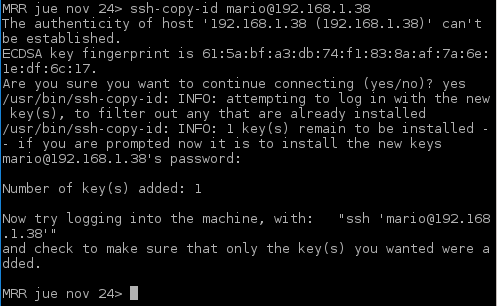
\includegraphics[scale=0.9]{figuras/figura98.png} 
	\caption{Copia de la clave en el host destino} 
	\label{fig:figura98}
\end{figure}

La clave publica generada en la máquina Centos, Figura \ref{fig:figura99}, es la que se encuentra en \textbf{\AC/.ssh/id\_ecdsa.pub} y que se ha enviado a la máquina Ubuntu.

\begin{figure}[H] %con el [H] le obligamos a situar aquí la figura
	\centering
	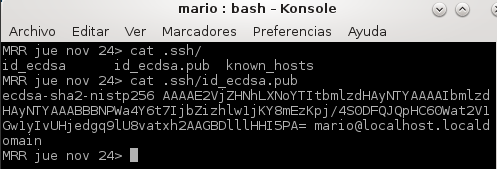
\includegraphics[scale=1]{figuras/figura99.png} 
	\caption{Contenido de la clave pública de Centos} 
	\label{fig:figura99}
\end{figure}

Se puede comprobar ahora en la máquina Ubuntu en el fichero \textbf{\AC/.ssh/authorized\_keys} cómo se encuentra la misma clave anterior. La Figura \ref{fig:figura100} muestra el contenido del fichero mencionado de Ubuntu.

\begin{figure}[H] %con el [H] le obligamos a situar aquí la figura
	\centering
	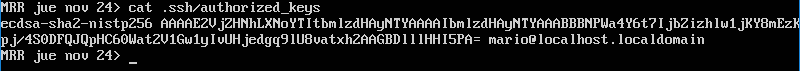
\includegraphics[scale=0.7]{figuras/figura100.png} 
	\caption{Clave de la máquina Centos dentro de Ubuntu} 
	\label{fig:figura100}
\end{figure}

\newpage

En la Figura \ref{fig:figura98} se ve cómo se ha requerido la contraseña de administrador de Ubuntu para conectarse desde Centos. Pues bien, esta ha sido la última vez que sucederá.
Prueba de ello existe en la Figura \ref{fig:figura101}

\begin{figure}[H] %con el [H] le obligamos a situar aquí la figura
	\centering
	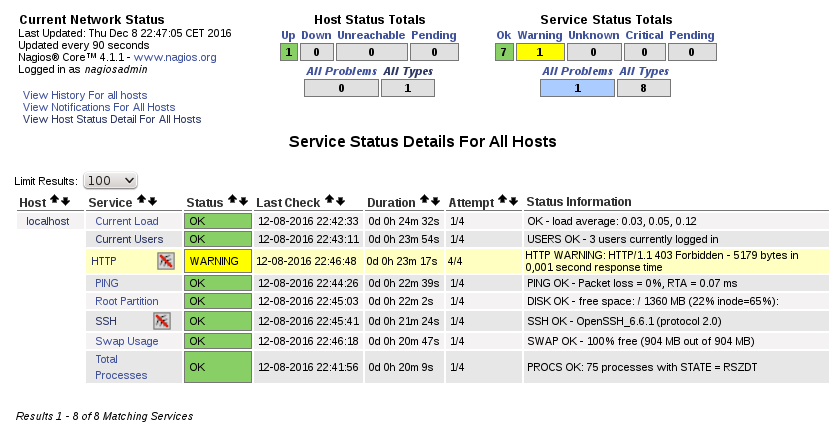
\includegraphics[scale=0.8]{figuras/figura20.png} 
	\caption{Conexión por ssh sin introducir contraseña} 
	\label{fig:figura101}
\end{figure}


\newpage

%----------------------------------------------------------------------------------------
%	Cuestión 7
%----------------------------------------------------------------------------------------
\section{Cuestión 7}
\subsection{¿Qué archivo es el que contiene la configuración del servicio
	ssh?}

El archivo que contiene la configuración del servicio ssh es \textbf{ /etc/ssh/sshd\_config} \cite{enlace19}. Parte de su contenido puede verse en la Figura \ref{fig:figura102}
	
	\begin{figure}[H] %con el [H] le obligamos a situar aquí la figura
		\centering
		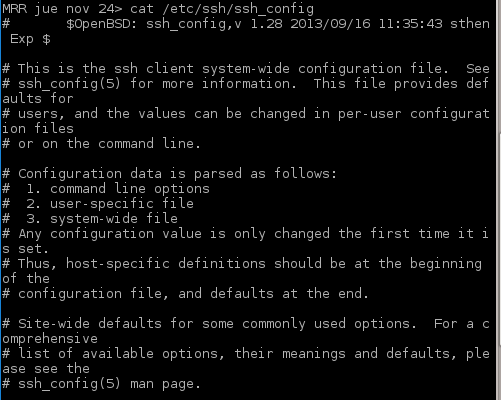
\includegraphics[scale=0.6]{figuras/figura102.png} 
		\caption{Fichero de configuración de ssh} 
		\label{fig:figura102}
	\end{figure}
\subsection{¿Qué parámetro hay que modificar para evitar que el usuario root
	acceda?}

El parámetro que hay que modificar para evitar que el usuario root acceda es 

\textit{PermitRootLogin}, su posición en el fichero puede verse en la Figura \ref{fig:figura103}

\begin{figure}[H] %con el [H] le obligamos a situar aquí la figura
	\centering
	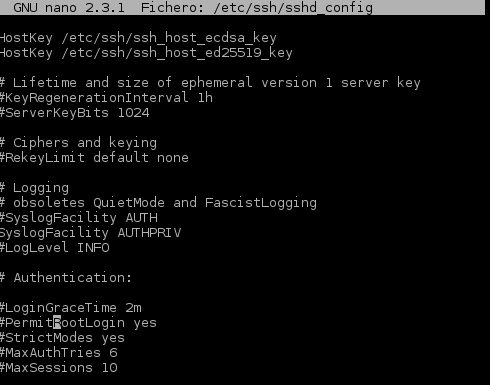
\includegraphics[scale=0.6]{figuras/figura103.png} 
	\caption{Conexión por ssh sin introducir contraseña} 
	\label{fig:figura103}
\end{figure}

 La modificación debe quedar así en el fichero:

\textbf{PermitRootLogin no}

\subsection{Cambie el puerto por defecto y compruebe que puede acceder}	

Para cambiar el puerto por defecto hay que modificar el valor de \textbf{Port} dentro del fichero \textbf{ /etc/ssh/sshd\_config}.

En ese fichero se ha cambiado su valor por el de 2222.
La Figura \ref{fig:figura104} muestra que se ha cambiado dicho valor a través de nano, a continuación se ha abierto el puerto nuevo y por último, por ipconfig aparece la IP de Centos que va a utilizar la máquina de Ubuntu para conectarse por ssh.
\begin{figure}[H] %con el [H] le obligamos a situar aquí la figura
	\centering
	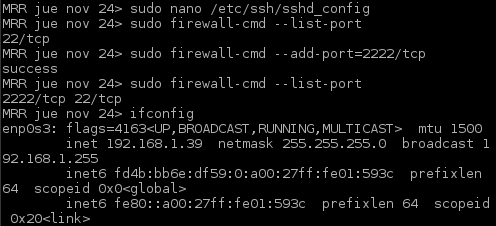
\includegraphics[scale=0.9]{figuras/figura104.png} 
	\caption{Cambio del puerto SSH a \textbf{2222} en Centos} 
	\label{fig:figura104}
\end{figure}

En la Figura \ref{fig:figura105} puede demostrarse que no ha habido nigún problema con el acceso después de hacer el cambio del valor del puerto.

\begin{figure}[H] %con el [H] le obligamos a situar aquí la figura
	\centering
	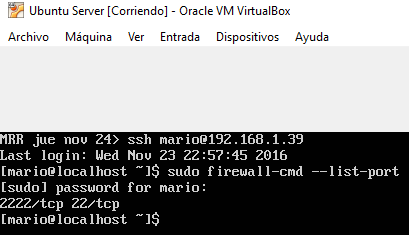
\includegraphics[scale=0.9]{figuras/figura105.png} 
	\caption{Conexión de Ubuntu a Centos con nuevo puerto ssh} 
	\label{fig:figura105}
\end{figure}

\newpage

%----------------------------------------------------------------------------------------
%	Cuestión 8
%----------------------------------------------------------------------------------------
\section{Cuestión 8}
\subsection{Indique si es necesario reiniciar el servicio ¿Cómo se reinicia
	un servicio en Ubuntu?}	

Es necesario reiniciar el servicio si se quiere que los cambios sean válidos
en ese momento. De no ser así hay que esperar a un reinicio del sistema operativo para que los cambios realizados surjan efecto.

Para reiniciar el servicio en Ubuntu existen dos métodos distintos \cite{enlace20}:

\begin{enumerate}
	\item [$>$] \textbf{sudo service \textit{servicio} restart}
	\item [$>$] \textbf{sudo /etc/init.d/\textit{servicio} restart}
	\begin{figure}[H] %con el [H] le obligamos a situar aquí la figura
		\centering
		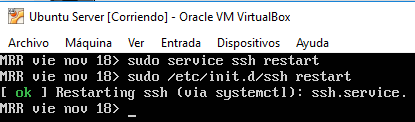
\includegraphics[scale=0.8]{figuras/figura22.png} 
		\caption{Reinicio del servicio \textbf{ssh} en Ubuntu} 
		\label{fig:figura22}
	\end{figure}
\end{enumerate}
\subsection{¿y en CentOS? Muestre la secuencia de comandos
	para hacerlo.}	

$ > $ \textbf{sudo service \textit{servicio} restart} \cite{enlace21}
\begin{figure}[H] %con el [H] le obligamos a situar aquí la figura
	\centering
	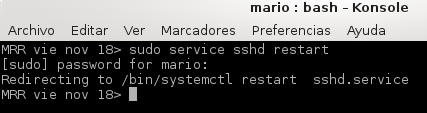
\includegraphics[scale=0.8]{figuras/figura23.png} 
	\caption{Reinicio del servicio \textbf{ssh} en CentOS} 
	\label{fig:figura23}
\end{figure}

\newpage

%----------------------------------------------------------------------------------------
%	Cuestión 9
%----------------------------------------------------------------------------------------
\section{Cuestión 9}
\textbf{\textit{Muestre los comandos que ha utilizado en Ubuntu Server y en
	CentOS (aunque en este último puede utilizar la GUI, en tal caso, realice
	capturas de pantalla). Compruebe que la instalación ha sido correcta.}}

\subsection{Ubuntu Server: Instalación de Apache + MySQL + PHP} \cite{enlace22}
\begin{enumerate}
	\item [$>$] \textbf{sudo apt-get install lamp-server\^}
	\item [$>$] \textbf{sudo service apache2 restart} 
\end{enumerate}

\subsection{CentOS: Instalación de Apache + MySQL + PHP} \cite{enlace23}

\subsubsection{Instalación MySQL /  MariaDB}
	\begin{itemize}
		\item Orden para la instalación a través de la linea de comandos, Figura \ref{fig:figura28}:
		\begin{figure}[H] %con el [H] le obligamos a situar aquí la figura
			\centering
			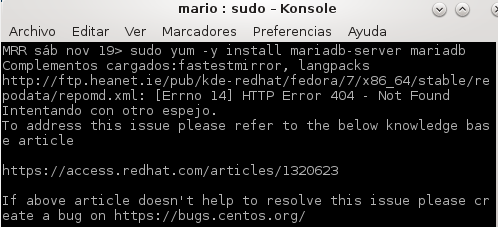
\includegraphics[scale=0.5]{figuras/figura28.png} 
			\caption{Instalación de MySQL $ / $ MariaDB} 
			\label{fig:figura28}
		\end{figure}
	
		\item Configuración de arranque inicial en el sistema y de la cuenta root, Figura \ref{fig:figura29}:
		\begin{figure}[H] %con el [H] le obligamos a situar aquí la figura
			\centering
			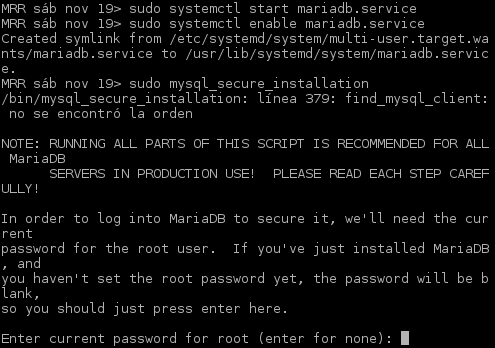
\includegraphics[scale=0.6]{figuras/figura29.png} 
			\caption{Configuración de la cuenta root de MySQL} 
			\label{fig:figura29}
		\end{figure}
	\end{itemize}
		
	
\subsubsection{Instalación de Apache2}
	\begin{itemize}
		\item Orden para la instalación a través de la linea de comandos, Figura \ref{fig:figura30}:
		\begin{figure}[H] %con el [H] le obligamos a situar aquí la figura
			\centering
			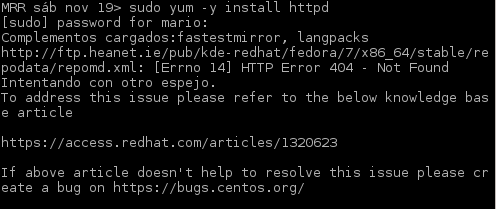
\includegraphics[scale=0.6]{figuras/figura30.png} 
			\caption{Instalación de Apache2} 
			\label{fig:figura30}
		\end{figure}
	
		\item Configuración de arranque inicial en el sistema y apertura de los puertos necesarios, Figura \ref{fig:figura31}:
		\begin{figure}[H] %con el [H] le obligamos a situar aquí la figura
			\centering
			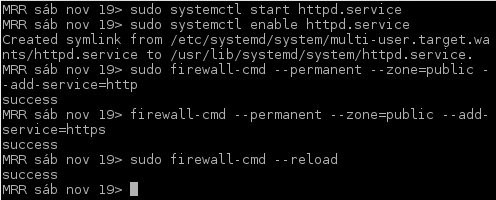
\includegraphics[scale=0.6]{figuras/figura31.png} 
			\caption{Configuración de arranque y apertura de puertos Apache} 
			\label{fig:figura31}
		\end{figure}
	
		\item Prueba del funcionamiento desde el navegador, Figura \ref{fig:figura32}:
		\begin{figure}[H] %con el [H] le obligamos a situar aquí la figura
			\centering
			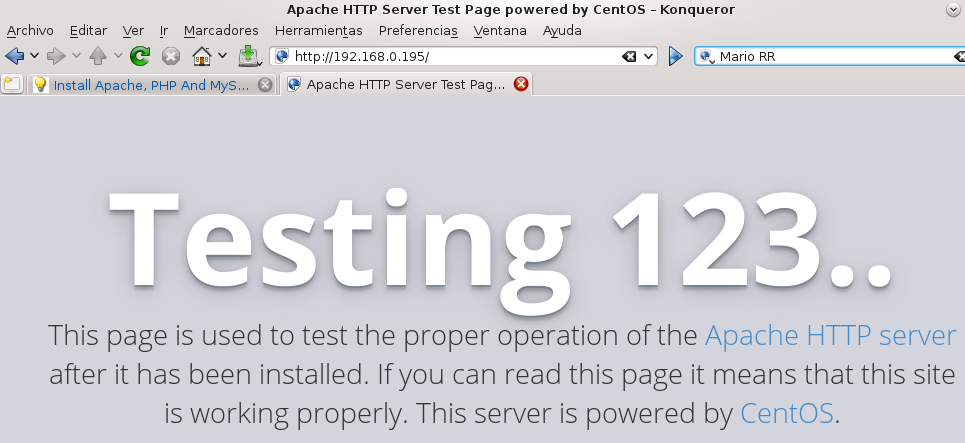
\includegraphics[scale=0.6]{figuras/figura32.png} 
			\caption{Prueba de Apache en el navegador} 
			\label{fig:figura32}
		\end{figure}
	\end{itemize}
			

\newpage

\subsubsection{Instalación de PHP5}
	\begin{itemize}
		\item Orden para la instalación a través de la linea de comandos, Figura \ref{fig:figura33}:
		\begin{figure}[H] %con el [H] le obligamos a situar aquí la figura
			\centering
			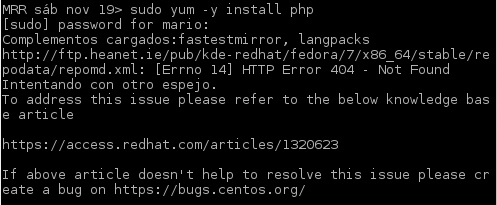
\includegraphics[scale=0.6]{figuras/figura33.png} 
			\caption{Instalación de PHP5} 
			\label{fig:figura33}
		\end{figure}
		
		\item Creación de un fichero PHP5 para su posterior prueba, Figura \ref{fig:figura34}:
		\begin{figure}[H] %con el [H] le obligamos a situar aquí la figura
			\centering
			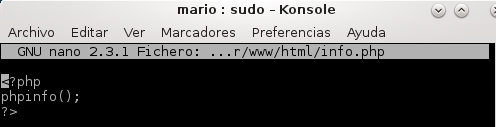
\includegraphics[scale=0.6]{figuras/figura34.png} 
			\caption{Creación de un fichero PHP5} 
			\label{fig:figura34}
		\end{figure}
	
		\item Prueba del funcionamiento desde el navegador, Figura \ref{fig:figura35}:
		\begin{figure}[H] %con el [H] le obligamos a situar aquí la figura
			\centering
			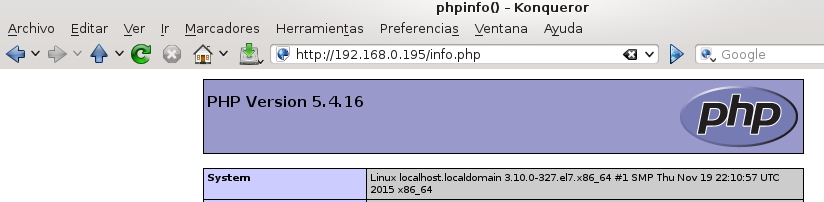
\includegraphics[scale=0.6]{figuras/figura35.png} 
			\caption{Prueba de PHP5 en el navegador} 
			\label{fig:figura35}
		\end{figure}
	\end{itemize}
	

\newpage

%----------------------------------------------------------------------------------------
%	Cuestión 10
%----------------------------------------------------------------------------------------
\section{Cuestión 10}
\subsection{Realice la instalación usando GUI o PowerShell}
	
	Se ha realizado la instalación usando GUI \cite{enlace23}.
	El proceso de instalación realizado usando el asistente para agregar roles y características puede verse en la Figura \ref{fig:figura36}:
	\begin{figure}[H]	
		\centering	
		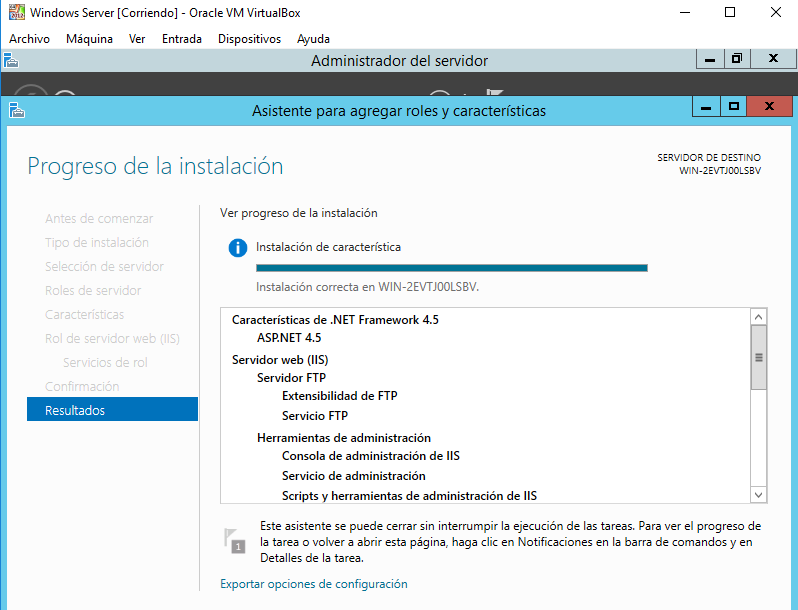
\includegraphics[scale=0.4]{figuras/figura36.png} 
		\caption{Proceso de instalación del IIS en Windows Server} 
		\label{fig:figura36}
	\end{figure}

	Una vez terminada la instalación puede comprobarse que el servicio funciona a través del navegador web, poniendo en la barra de direcciones \textbf{http://localhost/}, como se hace en la Figura \ref{fig:figura37}
	\begin{figure}[H]
		\centering
		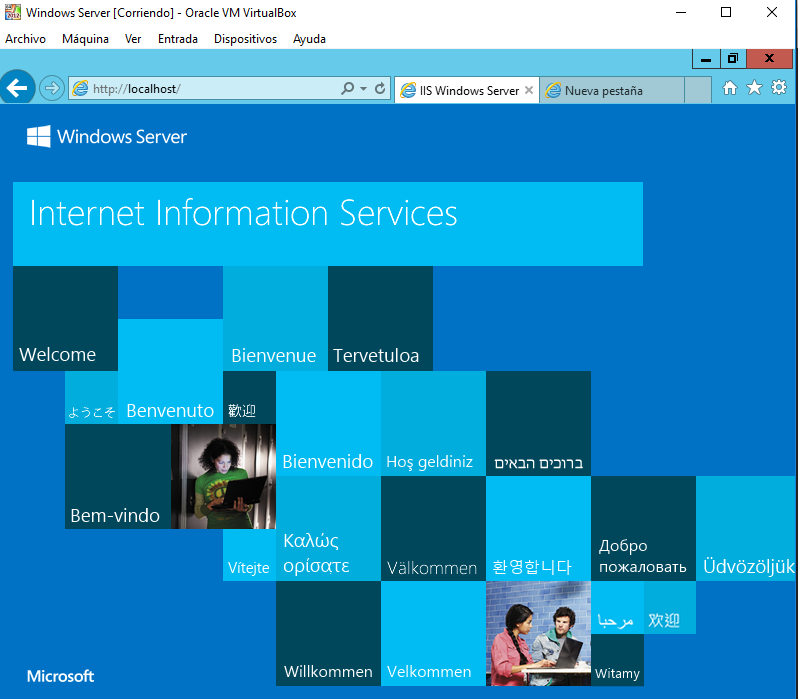
\includegraphics[scale=0.4]{figuras/figura37.png} 
		\caption{Prueba del servidor web en Windows Server} 
		\label{fig:figura37}
	\end{figure}

\subsection{Compruebe
	que el servicio está funcionando accediendo a la MV a través de la
	anfitriona}		
		
		En la parte izquierda de la Figura \ref{fig:figura38} se muestra la información de la lista de IPs para comprobar la dirección IP de la MV que hay que utilizar para conectarse a ella.
		
		En la parte derecha de la misma puede verse utilizada dicha IP en el host anfitrión, comprobando que el servicio funciona correctamente 
		
		\begin{figure}[H] %con el [H] le obligamos a situar aquí la figura
			\centering
			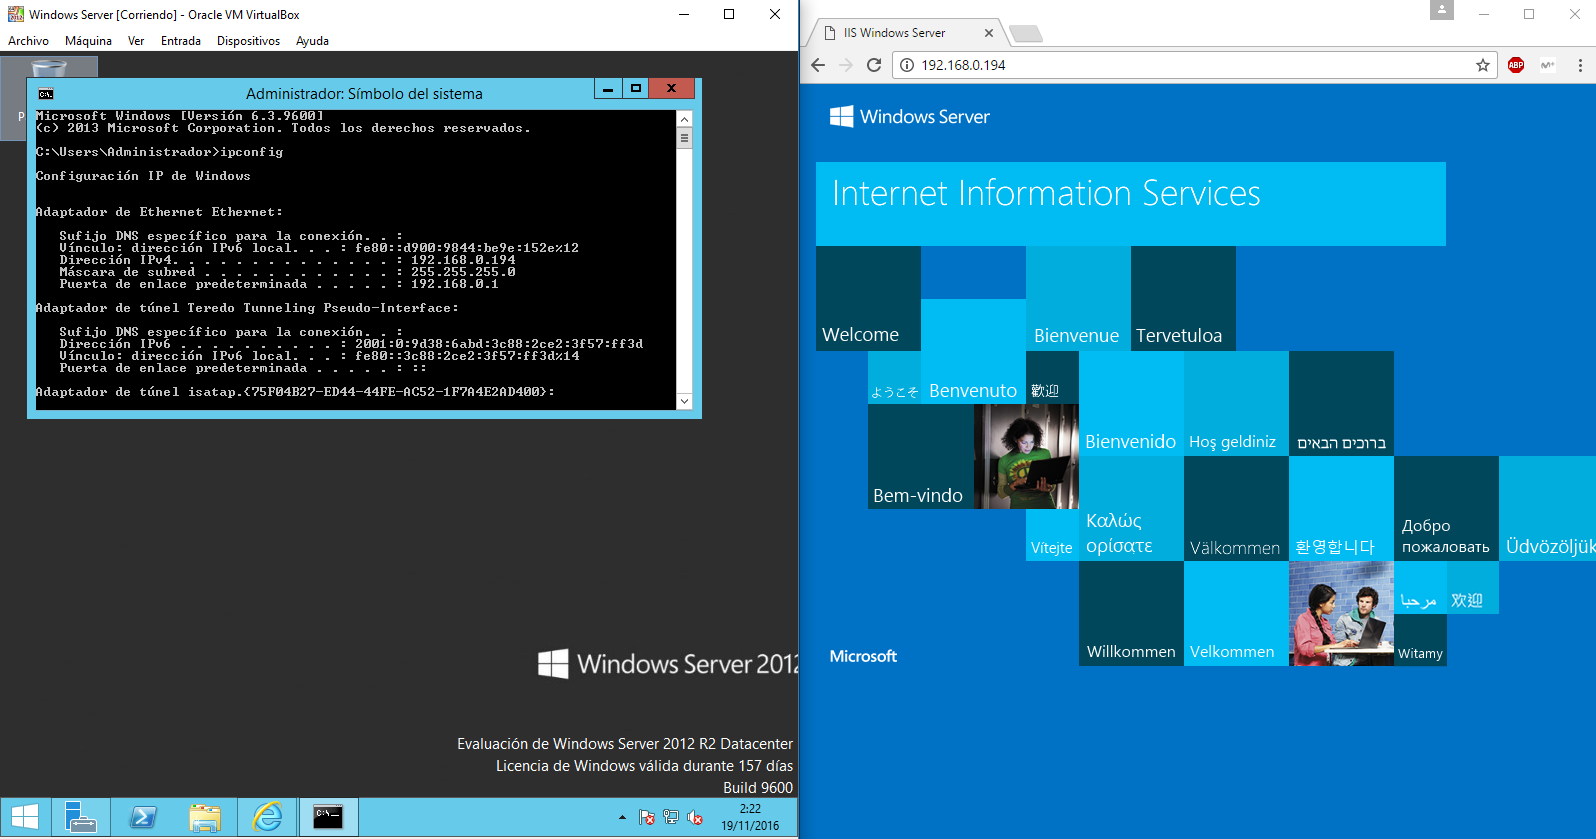
\includegraphics[scale=0.4]{figuras/figura38.png} 
			\caption{Prueba del servidor web (MV) desde la anfitriona} 
			\label{fig:figura38}
		\end{figure}

	
	

\newpage

%----------------------------------------------------------------------------------------
%	Cuestión 11
%----------------------------------------------------------------------------------------
\section{Cuestión 11}
\subsection{Muestre un ejemplo de uso del comando (p.ej.
http://fedoraproject.org/wiki/VMWare)}

Hay ocasiones en las que algunas características no están incluidas en el kernel estándar debido a la falta de desarrollo o de un posible desacuerdo con los desarrolladores del mismo. Tales características pueden ser distribuidas en forma de parches.
\\

Debian distribuye algunos de estos parches en paquetes linux-patch-* o kernel-patch-* . Estos paquetes se instalan los archivos en el \textbf{/usr/src/kernel-patches/}.
\\

Una vez conocidos los detalles del uso de patch, se aplicará el patch \textbf{grsecurity2} a un kernel en Debian \cite{enlace24} mediante las siguientes órdenes:
\begin{enumerate}
	\item [$>$]  \textbf{cd \AC/kernel/linux-source-3.16}
	\item [$>$] \textbf{make clean}
	\item [$>$] \textbf{zcat /usr/src/kernel-patches/diffs/grsecurity2/grsecurity-3.0-3.17.1-}
	
	\textbf{201410250027.patch.gz | patch -p1}
\end{enumerate}

\newpage

%----------------------------------------------------------------------------------------
%	Cuestión 12
%----------------------------------------------------------------------------------------
\section{Cuestión 12}
\textbf{\textit{Realice la instalación de esta aplicación y pruebe a modificar
	algún parámetro de algún servicio. Muestre las capturas de pantalla
	pertinentes así como el proceso de instalación.}}

\subsection{Instalación de Webmin en CentOS} \cite{enlace25}

\begin{itemize}
	\item Creación de un fichero tipo \textit{webmin.repo} en \textbf{/etc/yum.repos.d/}, Figura \ref{fig:figura39}:
	\begin{figure}[H] %con el [H] le obligamos a situar aquí la figura
		\centering
		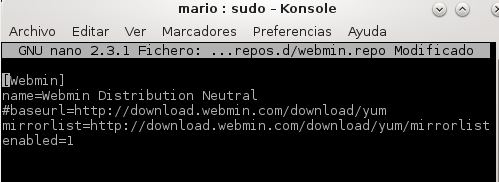
\includegraphics[scale=0.7]{figuras/figura39.png} 
		\caption{Creación de \textbf{/etc/yum.repos.d/webmin.repo}} 
		\label{fig:figura39}
	\end{figure}
	
	\item Instalación de la clave GPC Webmin y de la herramienta, Figura \ref{fig:webm}:
	\begin{figure}[htbp]
		\centering
		\begin{subfigure}[H]{0.3\textwidth}		
			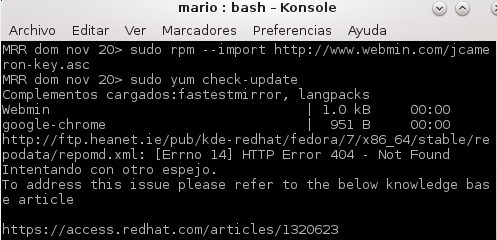
\includegraphics[scale=0.4]{figuras/figura40.png} 
			\caption{Instalación de la clave GPC} 
			\label{fig:figura40}
		\end{subfigure}	\hspace{20mm}
		\begin{subfigure}[H]{0.5\textwidth}
			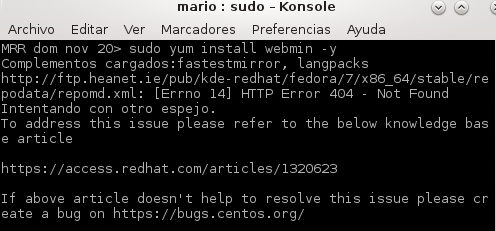
\includegraphics[scale=0.4]{figuras/figura41.png} 
			\caption{Instalación de la herramienta Webmin} 
			\label{fig:figura41}
		\end{subfigure}
		\caption{Instalación de la clave GPC Webmin y de la herramienta.} \label{fig:webm}
	\end{figure}

	\item Inicio, automatización del servicio y apertura del puerto necesario (\textbf{10000/tcp}), Figura \ref{fig:figura42}:
	\begin{figure}[H] %con el [H] le obligamos a situar aquí la figura
		\centering
		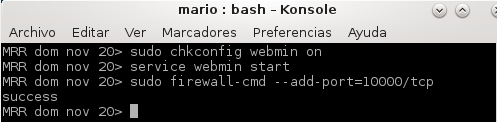
\includegraphics[scale=0.8]{figuras/figura42.png} 
		\caption{Inicio, automatización del servicio y apertura del puerto necesario para Webmin} 
		\label{fig:figura42}
	\end{figure}

\newpage

\subsection{Ejecución de Webmin en CentOS}
	\item Inicio de la herramienta desde el navegador:
	
		Acceso mediante los datos de administrador, , Figura \ref{fig:figura43}.
	\begin{figure}[H] %con el [H] le obligamos a situar aquí la figura
		\centering
		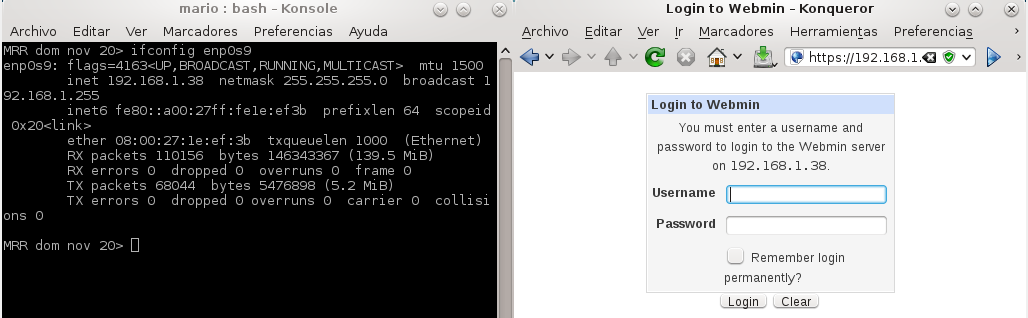
\includegraphics[scale=0.6]{figuras/figura43.png} 
		\caption{Inicio de Webmin a través del navegador.} 
		\label{fig:figura43}
	\end{figure}

	\item Información del sistema, Figura \ref{fig:figura44}:
	\begin{figure}[H] %con el [H] le obligamos a situar aquí la figura
		\centering
		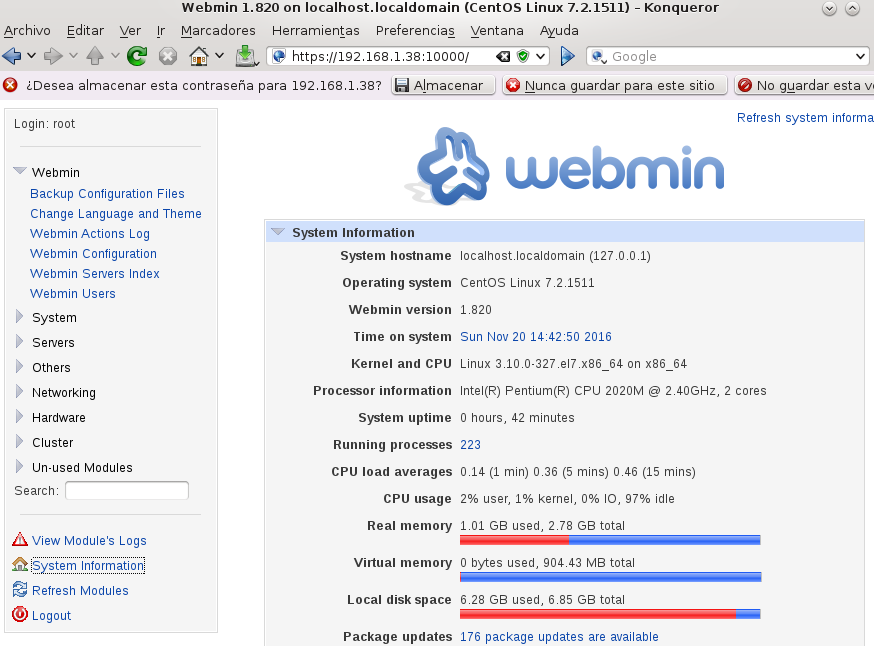
\includegraphics[scale=0.6]{figuras/figura44.png} 
		\caption{Información del sistema desde Webmin} 
		\label{fig:figura44}
	\end{figure}

\newpage

\subsection{Apertura de puertos en CentOS desde Webmin}

	\item Apertura de puertos, Figura \ref{fig:figura45}:
	\begin{figure}[H] %con el [H] le obligamos a situar aquí la figura
		\centering
		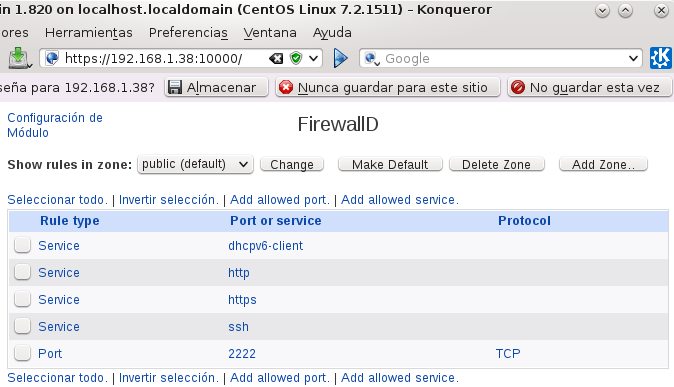
\includegraphics[scale=0.7]{figuras/figura45.png} 
		\caption{Puertos abiertos en el sistema} 
		\label{fig:figura45}
	\end{figure}

	\item Apertura del puerto necesario para \textbf{telnet}:
	
	Prueba de la apertura de un puerto para verificar el funcionamiento de la herramienta, Figura \ref{fig:webc}.
	\begin{figure}[htbp]
		\centering
		\begin{subfigure}[H]{0.3\textwidth}		
			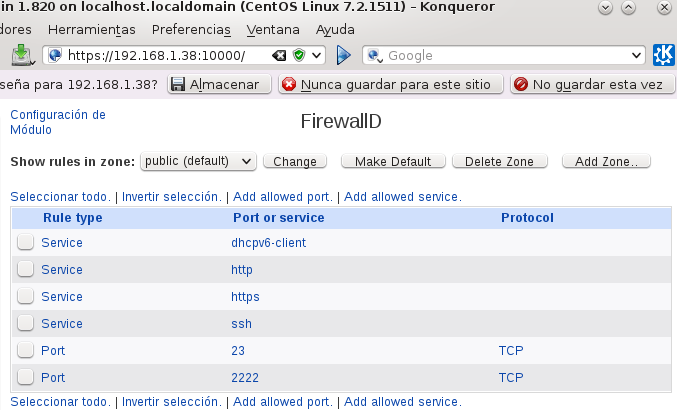
\includegraphics[scale=0.4]{figuras/figura46.png} 
			\caption{Apertura del puerto 23 desde Webmin} 
			\label{fig:figura46}
		\end{subfigure}	\hspace{30mm}
		\begin{subfigure}[H]{0.3\textwidth}
			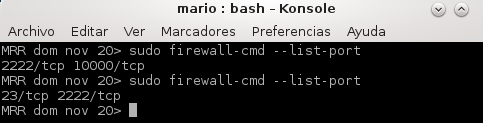
\includegraphics[scale=0.5]{figuras/figura47.png} 
			\caption{Listado de puertos abiertos desde consola} 
			\label{fig:figura47}
		\end{subfigure}
		\caption{Apertura del puerto de telnet desde Webmin} 
		\label{fig:webc}	
	\end{figure}
	
	En la Figura \ref{fig:webc} puede verse el listado de puertos desde consola antes y después de la modificación a través de Webmin.
\end{itemize}


\newpage

%----------------------------------------------------------------------------------------
%	Cuestión 13
%----------------------------------------------------------------------------------------
\section{Cuestión 13}
\textbf{\textit{Instale phpMyAdmin, indique cómo lo ha realizado y muestre
algunas capturas de pantalla. Configure PHP para poder importar BDs de
hasta 25MiB (en vez de los 8 MiB de límite por defecto). Indique cómo ha
realizado el proceso y muestre capturas de pantalla.}}
\\

\subsection{Instalación de phpMyAdmin en CentOS}
\cite{enlace23,enlace25}

\begin{enumerate}
	\item Instalación de phpMyAdmin en CentOS:
	
	\begin{figure}[H] %con el [H] le obligamos a situar aquí la figura
		\centering
		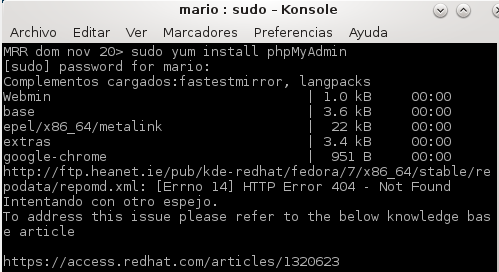
\includegraphics[scale=0.7]{figuras/figura48.png} 
		\caption{Orden para la instalación de phpMyAdmin en CentOS} 
		\label{fig:figura48}
	\end{figure}
	
	En el caso de que la instalación de la herramienta se realizara de forma remota habría que cambiar la IP que trae por defecto en el fichero de configuración \textbf{/etc/httpd/conf.d/phpMyAdmin.conf} a través de las lineas siguientes, como las que aparecen en la Figura \ref{fig:figura49}:
	\\
	
	\textbf{Require ip \textit{ IP\_address }}
	
	\textbf{Allow from \textit{ IP\_address }}
	\\
	
	En IP\_address irá la IP del host desde donde accedemos remotamente.
	Puede consultarse, por ejemplo, desde  \url{http://www.cualesmiip.com/} 
	\\
	
	NOTA: Esta última parte es solamente informativa, en este caso se va a realizar de forma local.
	
	\begin{figure}[H] %con el [H] le obligamos a situar aquí la figura
		\centering
		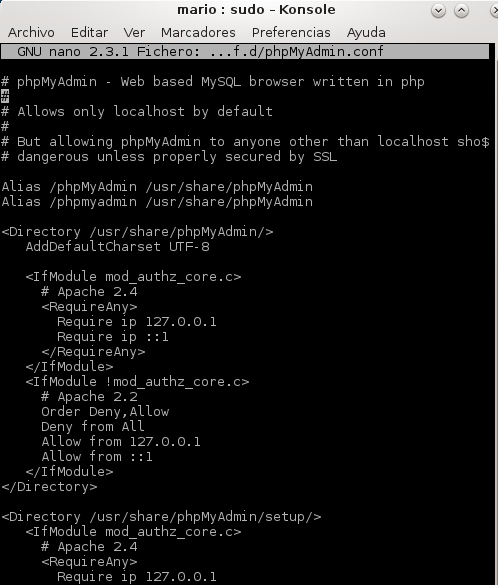
\includegraphics[scale=0.6]{figuras/figura49.png} 
		\caption{Cambio de la IP para acceder de forma remota a phpMyAdmin} 
		\label{fig:figura49}
	\end{figure}

	\item Reinicio del servicio Apache para efectuar los cambios:
	\item[$ > $] \textbf{sudo service httpd restart}
	
	\item Inicio de phpMyAdmin desde el navegador en \textbf{http://localhost/phpmyadmin/}:
	
	Para identificarse hay que utilizar los datos de administrador como en la Figura \ref{fig:figura52}.
	
	\begin{figure}[H] %con el [H] le obligamos a situar aquí la figura
		\centering
		\includegraphics[scale=0.4]{figuras/figura52.png} 
		\caption{Inicio y autentificación en phpMyAdmin} 
		\label{fig:figura52}
	\end{figure}
	
	\item Prueba del servicio, algo parecido al contenido de la Figura \ref{fig:figura53}.:
		
	\begin{figure}[H] %con el [H] le obligamos a situar aquí la figura
		\centering
		\includegraphics[scale=0.6]{figuras/figura53.png} 
		\caption{Pantalla principal de phpMyAdmin} 
		\label{fig:figura53}
	\end{figure}
	
\end{enumerate}

\subsection{Configuración de PHP para importar BDs de
	hasta 25MiB}
\cite{enlace26}

Como se aprecia en la Figura \ref{fig:figura55} el tamaño máximo para importar BDs es de 2MB.

\begin{figure}[H] %con el [H] le obligamos a situar aquí la figura
	\centering
	\includegraphics[scale=0.6]{figuras/figura55.png} 
	\caption{Tamaño máximo inicial de archivos a importar en phpMyAdmin} 
	\label{fig:figura55}
\end{figure}

\newpage

Para poder importar BDs de hasta 25MiB hay que modificar dos lineas del fichero de configuración \textbf{/etc/php.ini}:

\textbf{upload\_max\_filesize = 25M}

\textbf{post\_max\_size = 25M}

\begin{figure}[H] %con el [H] le obligamos a situar aquí la figura
	\centering
	\includegraphics[scale=0.9]{figuras/figura54.png} 
	\caption{Fichero de configuración de phpMyAdmin} 
	\label{fig:figura54}
\end{figure}

Por último, para que los cambios realizados puedan verse efectuados hay que reiniciar el servicio Apache.
Para ello basta con ejecutar la orden siguiente por consola:
\\

$ > $ \textbf{sudo service httpd restart}

\begin{figure}[H] %con el [H] le obligamos a situar aquí la figura
	\centering
	\includegraphics[scale=0.7]{figuras/figura56.png} 
	\caption{Tamaño máximo actualizado de archivos a importar en phpMyAdmin} 
	\label{fig:figura56}
\end{figure}

Ya puede apreciarse cómo ha cambiado el tamaño máximo del archivo de importación en la Figura \ref{fig:figura56}

\newpage

%----------------------------------------------------------------------------------------
%	Cuestión 14
%----------------------------------------------------------------------------------------
\section{Cuestión 14}
\textbf{\textit{Visite al menos una de las webs de los software mencionados
y pruebe las demos que ofrecen realizando capturas de pantalla y
comentando qué está realizando.}}
\\

La web visitada ha sido \url{http://www.ispconfig.org/}.

\begin{figure}[H] %con el [H] le obligamos a situar aquí la figura
	\centering
	\includegraphics[scale=0.5]{figuras/figura57.png} 
	\caption{Página principal de \textbf{ipsconfig}} 
	\label{fig:figura57}
\end{figure}

En primer lugar, para poder acceder a una demo hay que pulsar en la parte baja de la página principal en el botón $ " $Online Demo$ " $, como muestra la Figura \ref{fig:figura57}.

Una vez en dicho espacio, como lo que interesa es tener recursos de administrador, se pulsará el link \url{http://demo3.ispconfig.org/} que dará lugar a algo parecido a la Figura \ref{fig:figura58} y posteriormente se introducirán los siguientes datos para la identificación:
\\

Username: \textbf{admin}

Password: \textbf{demo}

\begin{figure}[H] %con el [H] le obligamos a situar aquí la figura
	\centering
	\includegraphics[scale=0.6]{figuras/figura58.png} 
	\caption{Login para administrador online demo en ipsconfig} 
	\label{fig:figura58}
\end{figure}

Introducidos los datos correctamente, aparecerá la página principal de la demo que ofrece el sitio. Algo como la Figura \ref{fig:figura59}

\begin{figure}[H] %con el [H] le obligamos a situar aquí la figura
	\centering
	\includegraphics[scale=0.4]{figuras/figura59.png} 
	\caption{Página principal de la demo de administrador de \textbf{ipsconfig}} 
	\label{fig:figura59}
\end{figure}

Tanto en la parte de arriba en forma de pestañas,
como en el cuerpo de la web, aparecen los módulos de configuración disponibles en este sistema. Si se elige
alguno producirá a una nueva pantalla de administración.
\\

A continuación se mostrará un ejemplo para añadir un nuevo cliente.

\newpage

Pulsando sobre \textit{Clients} y a continuación sobre \textit{Add client} aparecerá una ficha para rellenar como la de la Figura \ref{fig:figura60}

\begin{figure}[H] %con el [H] le obligamos a situar aquí la figura
	\centering
	\includegraphics[scale=0.4]{figuras/figura60.png} 
	\caption{Añadir un cliente en la demo de ipsconfig} 
	\label{fig:figura60}
\end{figure}

Una vez rellenos los datos, aceptados y aplicados por el sistema aparecerá el nuevo cliente en la lista de clientes. Véase la Figura \ref{fig:figura71}

\begin{figure}[H] %con el [H] le obligamos a situar aquí la figura
	\centering
	\includegraphics[scale=0.4]{figuras/figura71.png} 
	\caption{Lista de clientes actualizada en la demo de ipsconfig} 
	\label{fig:figura71}
\end{figure}

Una opción interesante que ofrece este sistema es la de \textbf{monitorización}.
Ésta hace que pueda sacarse un informe de errores organizados y clasificados en un tiempo de refresco específico para llevar un control en tiempo real del estado del servidor. Un ejemplo de ello es la Figura  \ref{fig:figura72}

\begin{figure}[H] %con el [H] le obligamos a situar aquí la figura
	\centering
	\includegraphics[scale=0.4]{figuras/figura72.png} 
	\caption{Estado del servidor en la demo online de ipsconfig}
	\label{fig:figura72}
\end{figure}

Es posible cambiar el idioma de sitio desde \textit{Tools} - \textit{Password and Language}, Figura \ref{fig:figura74} 

\begin{figure}[H] %con el [H] le obligamos a situar aquí la figura
	\centering
	\includegraphics[scale=0.3]{figuras/figura74.png} 
	\caption{Cambio de idioma de la demo de ipsconfig}
	\label{fig:figura74}
\end{figure}

Este cambio produce un error argumentando que esta función está deshabilitada para el modo demo pero, a pesar de ello, el idioma se modifica. En la Figura \ref{fig:figura75} puede apreciarse que ahora el idioma del sistema está en español.

\begin{figure}[H] %con el [H] le obligamos a situar aquí la figura
	\centering
	\includegraphics[scale=0.3]{figuras/figura75.png} 
	\caption{Cambio de idioma realizado de la demo de ipsconfig}
	\label{fig:figura75}
\end{figure}

\newpage

%-------------------------------------------------------------------------------------------
%	Cuestión 15
%----------------------------------------------------------------------------------------
\section{Cuestión 15}

\subsection{Ejecute los ejemplos de find, grep}

Los ejemplos aparecen en la Figura \ref{fig:figura76}.

En primer lugar se prueba el funcionamiento de \textbf{grep} en el que se muestra la información del proceso firefox (descartando el resto
de información).
\\

En segundo lugar se prueba \textbf{find}, que copiará todos los archivos cuyo nombre termine en pdf y los copia en
la carpeta /home/mario/PDFs

	\begin{figure}[H] %con el [H] le obligamos a situar aquí la figura
		\centering
		\includegraphics[scale=0.8]{figuras/figura76.png} 
		\caption{Prueba de ejecución de \textbf{find} y \textbf{grep}}
		\label{fig:figura76}
	\end{figure}
	
\subsection{Escriba el
	script que haga uso de sed para cambiar la configuración de ssh y
	reiniciar el servicio.}
\cite{enlace27}

	\lstinputlisting[language=csh]{fuentes/scriptSed.sh}
	
	El script modifica el puerto que tenga especificado el servicio ssh por uno pasado como argumento y, a continuación, reinicia el servicio.
	
\newpage

	El uso del script puede verse en la Figura \ref{fig:figura77}, en la que en primer lugar se comprueba que el puerto actual; a continuación se ejecuta el script y por último se comprueba que el puerto se haya modificado correctamente.
	
	\begin{figure}[H] %con el [H] le obligamos a situar aquí la figura
		\centering
		\includegraphics[scale=0.9]{figuras/figura77.png} 
		\caption{Script que cambia el puerto de ssh}
		\label{fig:figura77}
	\end{figure}

\subsection{Muestre un ejemplo de uso para awk}

Uso de \textbf{awk} \cite{enlace28} para mostrar todas las líneas del fichero \textbf{/etc/ssh/sshd\_config} cuyo segundo campo contenga el número \textbf{22}.
\\

$ > $ \textbf{awk '\$2 \AC /22/' /etc/ssh/sshd\_config}

Vista de la ejecución en la Figura \ref{fig:figura78}

\begin{figure}[H] %con el [H] le obligamos a situar aquí la figura
	\centering
	\includegraphics[scale=0.9]{figuras/figura78.png} 
	\caption{Script en Bash que cambia el puerto de ssh}
	\label{fig:figura78}
\end{figure}

\newpage

%-------------------------------------------------------------------------------------------
%	Cuestión 16
%----------------------------------------------------------------------------------------
\section{Cuestión 16}
\subsection{Escriba el script para cambiar el acceso a ssh usando
PHP o Python.}
\cite{enlace29}

\lstinputlisting[language=python]{fuentes/sshPython.py}

El script modifica el puerto que tenga especificado el servicio ssh por uno pasado como argumento y, a continuación, reinicia el servicio.

\newpage

El uso del script puede verse en la Figura \ref{fig:figura77}, en la que en primer lugar se comprueba que el puerto actual; a continuación se ejecuta el script y por último se comprueba que el puerto se haya modificado correctamente.

\begin{figure}[H] %con el [H] le obligamos a situar aquí la figura
	\centering
	\includegraphics[scale=0.9]{figuras/figura79.png} 
	\caption{Script en Python que cambia el puerto de ssh}
	\label{fig:figura79}
\end{figure}

\newpage

%-------------------------------------------------------------------------------------------
%	Cuestión 17
%----------------------------------------------------------------------------------------
\section{Cuestión 17}
\subsection{Abra una consola de Powershell y pruebe a parar un
programa en ejecución (p.ej), realice capturas de pantalla y comente
lo que muestra.}

El programa en ejecución que se va a parar es Internet Explorer. Como puede
apreciarse en la Figura \ref{fig:figura80} existen hasta tres procesos ejecutándose a la vez de la misma aplicación.

$ > $ \textbf{Get-Process}

\begin{figure}[H] %con el [H] le obligamos a situar aquí la figura
	\centering
	\includegraphics[scale=0.9]{figuras/figura80.png} 
	\caption{Información de los procesos en ejecución desde PowerShell}
	\label{fig:figura80}
\end{figure}

Mediante la orden \textbf{Stop-Process -ID \textit{proceso}} se puede parar el proceso que se desee. En este caso se pararán los procesos 1468, 1900 y 2636, que son los que mantienen a Internet Explorer.

\newpage

Una vez realizadas dichas órdenes, en la Figura \ref{fig:figura81} puede verse cómo han desaparecido los procesos que nos interesaban.

\begin{figure}[H] %con el [H] le obligamos a situar aquí la figura
	\centering
	\includegraphics[scale=0.8]{figuras/figura81.png} 
	\caption{Parada de procesos desde PowerShell}
	\label{fig:figura81}
\end{figure}

Ha salido un error en la última orden porque el proceso ya no se encontraba disponible. Esto es porque dependía de alguno de los otros procesos que se habían eliminado antes que él y ha sido borrado de forma análoga. 

\newpage


%----------------------------------------------------------------------------------------
%	Cuestión opcional 2
%----------------------------------------------------------------------------------------
\section{Cuestión opcional 2}
\textbf{\textit{Para evitar ataques de fuerza bruta podemos usar fail2ban que mete en una
lista negra las IPs que intentan iniciar sesión de manera errónea.}}

\textbf{\textit{Instale el servicio y pruebe su funcionamiento.}} \cite{enlace21}

\begin{enumerate}
	\item Instalación del servicio:
	
	$ > $ \textbf{sudo yum install fail2ban}
	
	\item Por motivos de seguridad, hay que configurar un fichero local de configuración a través de una copia del original:
	
	$ > $ \textbf{sudo cp -pf   /etc/fail2ban/jail.conf   /etc/fail2ban/jail.local }
	
	\item Modificación del fichero de configuración local según intereses:
	
	$ > $ \textbf{sudo nano  /etc/fail2ban/jail.local }
	
	En este caso, para probar se han realizado las siguientes de la Figura \ref{fig:figura25}:
	
	\begin{figure}[H] %con el [H] le obligamos a situar aquí la figura
		\centering
		\includegraphics[scale=0.7]{figuras/figura25.png} 
		\caption{Fichero de configuración  /etc/fail2ban/jail.local } 
		\label{fig:figura25}
	\end{figure}

	\item Añadido de un archivo jail para proteger SSH, Figura \ref{fig:figura26}:
	
	$ > $ \textbf{sudo nano /etc/fail2ban/jail.d/sshd.local }
	
	\begin{figure}[H] %con el [H] le obligamos a situar aquí la figura
		\centering
		\includegraphics[scale=0.7]{figuras/figura26.png} 
		\caption{Archivo jail de protección SSH} 
		\label{fig:figura26}
	\end{figure}

	\item Reinicio del servicio para que se efectúen los cambios.
	
	$ > $ \textbf{sudo service fail2ban restart}
	
	\newpage
	
	\item Prueba de funcionamiento.
	
	En la Figura \ref{fig:figura24} se muestra cómo a los dos intentos
	ya se no posibilita la conexión.
	\begin{figure}[H] %con el [H] le obligamos a situar aquí la figura
		\centering
		\includegraphics[scale=0.9]{figuras/figura24.png} 
		\caption{Prueba de funcionamiento con fuerza bruta} 
		\label{fig:figura24}
	\end{figure}
	
	En la Figura \ref{fig:figura27} se puede comprobar la IP que acaba de ser baneada.
	\begin{figure}[H] %con el [H] le obligamos a situar aquí la figura
		\centering
		\includegraphics[scale=0.7]{figuras/figura27.png} 
		\caption{Prueba de funcionamiento con fuerza bruta} 
		\label{fig:figura27}
	\end{figure}
\end{enumerate}

\newpage

%----------------------------------------------------------------------------------------
%	Cuestión opcional 3
%----------------------------------------------------------------------------------------
\section{Cuestión opcional 3}
\textbf{\textit{Instale el servicio RKhunter y pruebe su funcionamiento}} \cite{enlace30}

\begin{itemize}
	
	\item Instalación del servicio RKhunter en Ubuntu Server.
	
	Por medio del comando:
	\\
	
	$ > $ \textbf{sudo apt-get install rkhunter}	
		
	\begin{figure}[H] %con el [H] le obligamos a situar aquí la figura
		\centering
		\includegraphics[scale=0.6]{figuras/figura82.png} 
		\caption{Instalación del servicio RKhunter en Ubuntu Server} 
		\label{fig:figura82}
	\end{figure}

	Después de ejecutar la orden de instalación (Figura \ref{fig:figura82}), aparecerá una ventana de configuración Postfix (Figura \ref{fig:figura83})
	en la que habrá que escoger el tipo de configuración del servidor de correo. La elección se hará en función de las necesidades.
	
	\begin{figure}[H] %con el [H] le obligamos a situar aquí la figura
		\centering
		\includegraphics[scale=0.5]{figuras/figura83.png} 
		\caption{Configuración Postfix en Rhunter} 
		\label{fig:figura83}
	\end{figure}

	Una vez finalizada la instalación, hay que actualizar los archivos de la base de datos del servicio. Estos archivos contienen información para determinar si el comportamiento de un fichero es sospechoso o no.
	
	Para ello se ejecutará la siguiente orden (Figura \ref{fig:figura84}):
	\\
	
	$ > $ \textbf{sudo rkhunter --propupd}
	
	\begin{figure}[H] %con el [H] le obligamos a situar aquí la figura
		\centering
		\includegraphics[scale=0.8]{figuras/figura84.png} 
		\caption{Actualización de la base de datos de Rhunter} 
		\label{fig:figura84}
	\end{figure}
	
	Además se comprobará que no existe una versión más reciente del servicio (Figura \ref{fig:figura84}) mediante el comando:
	
	$ > $ \textbf{sudo rkhunter --versioncheck}
	\\
	
	Ahora es el momento de ejecutar el servicio por vez primera, una forma de hacerlo es a través de la orden (Figura \ref{fig:figura85}):
	
	$ > $ \textbf{sudo rkhunter --checkall}
	
	\begin{figure}[H] %con el [H] le obligamos a situar aquí la figura
		\centering
		\includegraphics[scale=0.7]{figuras/figura85.png} 
		\caption{Primera ejecución de Rhunter} 
		\label{fig:figura85}
	\end{figure}

\newpage

	 La primera ejecución puede dar algunos mensajes de advertencia, pero no tiene por qué estar el sistema infectado. Un ejemplo de ello es lo que aparece en la Figura \ref{fig:figura86}
	 
	 \begin{figure}[H] %con el [H] le obligamos a situar aquí la figura
	 	\centering
	 	\includegraphics[scale=0.5]{figuras/figura86.png} 
	 	\caption{Advertencias en la ejecución Rhunter} 
	 	\label{fig:figura86}
	 \end{figure}
 
	 Para evitar estas advertencias, se puede reconfigurar rkhunter para que la próxima vez que se ejecute haga caso omiso de estos archivos a través de listas blancas. Esto se hace editando el archivo \textbf{/etc/rkhunter.conf} y quitando el \textbf{\#} de delante de estas líneas.
	 
	 \begin{figure}[H] %con el [H] le obligamos a situar aquí la figura
	 	\centering
	 	\includegraphics[scale=0.4]{figuras/figura87.png} 
	 	\caption{Resultados de la ejecución de Rhunter} 
	 	\label{fig:figura87}
	 \end{figure}
	 
	 En la Figura \ref{fig:figura87} pueden verse los resultados de la ejecución de rhunter. En este caso no se ha encontrado ningún rootkit en el sistema.
	 
	 Para más detalles sobre advertencias y demás puede visualizarse el log de la ejecución desde el fichero \textbf{/var/log/rkhunter.log}
	 
\end{itemize}

\newpage

%----------------------------------------------------------------------------------------
%	Cuestión opcional 5
%----------------------------------------------------------------------------------------
\section{Cuestión opcional 5}
\cite{enlace31}
\subsection{Realice la instalación de MongoDB en alguna de sus
	máquinas virtuales.} 

\begin{itemize}
	\item Instalación de MongoDB en Centos 7:
	
	El paquete de instalación de Mongo no existe dentro de los repositorios por defecto de Centos. A pesar de ello MongoDB dispone de un repositorio dedicado que se puede añadir al servidor.
	
	Para ello se añade la información del repositorio con nombre \textbf{/etc/yum.repos.d/mongodb-org.repo}. A continuación se añadirán las lineas que aparecen en la Figura \ref{fig:figura88}.
	
	\begin{figure}[H] %con el [H] le obligamos a situar aquí la figura
		\centering
		\includegraphics[scale=0.5]{figuras/figura88.png} 
		\caption{Fichero de configuración del repositorio de MongoDB} 
		\label{fig:figura88}
	\end{figure}

	Ahora se comprobará que el repositorio ya existe en sistema a través de la orden \textbf{yum repolist} (Figura \ref{fig:figura89}), y seguidamente se procederá a su instalación mediante el comando:
	\\
	
	$ > $ \textbf{sudo yum install mongodb-org}
	
	\begin{figure}[H] %con el [H] le obligamos a situar aquí la figura
		\centering
		\includegraphics[scale=0.5]{figuras/figura89.png} 
		\caption{Instalación de MongoDB en Centos 7} 
		\label{fig:figura89}
	\end{figure}
\end{itemize}

\subsection{Cree una colección de documentos y haga una consulta
	sobre ellos.}
	
	La colección de documentos en MongoDB debe tener una estructura similar a la de aquí abajo y tendrá extensión \textbf{.json}
	\\
	
	En esta ocasión se ha creado una colección con datos de algunas de las facultades de Granada, fichero nombrado como \textbf{colecciones.json}.
	
	\begin{lstlisting}
	{"direccion": 
		{"building": "2", 
		"coord": [-76.856077, 53.848447], 
		"calle": "Periodista Daniel Saucedo", 
	"zipcode": "10462"}, 
	"borough": "Granada", 
	"tipo": "Ingeniería", 
	"name": "ETSIIT", 
	"universidad_id": "30075441"}
	{"direccion": 
		{"building": "3", 
		"coord": [-36.856077, 20.848447], 
		"calle": "Puentezuelas", 
		"zipcode": "10462"}, 
	"borough": "Granada", 
	"tipo": "Letras", 
	"name": "Facultad de Traducción e Interpretación", 
	"universidad_id": "30075442"}
	{"direccion": 
		{"building": "4", 
		"coord": [-47.856077, 98.848447], 
		"calle": "Avenida de Andalucía", 
		"zipcode": "10462"}, 
	"borough": "Granada", 
	"tipo": "Ingeniería", 
	"name": "Facultad de Arquitectura", 
	"universidad_id": "30075443"}
	\end{lstlisting}

	Una vez creada la colección hay que importarla a Mongo. Para ello se utiliza la siguiente orden:
	
	$ > $ \textbf{mongoimport --db test --collection \textit{nombreColección} --file \textit{ficheroColeccion}.json}
	\\
	
	Puede ver su ejecución en la Figura \ref{fig:figura93}
	
	\begin{figure}[H] %con el [H] le obligamos a situar aquí la figura
		\centering
		\includegraphics[scale=0.7]{figuras/figura93.png} 
		\caption{Guardado de una colección en Mongo} 
		\label{fig:figura93}
	\end{figure}

	Una vez guardada la colección, puede ejecutarse el servicio Mongo para consultar cualquier dato sobre ésta.
	
	En esta ocasión se ha procedido a buscar dentro de la colección \textbf{universidades}, con el límite de \textbf{un documento} y en modo \textbf{pretty} (muestra tabulados los datos). Véase la Figura \ref{fig:figura94} 
	
	\begin{figure}[H] %con el [H] le obligamos a situar aquí la figura
		\centering
		\includegraphics[scale=1]{figuras/figura94.png} 
		\caption{Consulta de documentos de una colección en Mongo} 
		\label{fig:figura94}
	\end{figure}
	
\newpage

%----------------------------------------------------------------------------------------
%	Referencias
%----------------------------------------------------------------------------------------
%------------------------------------------------

\bibliography{citas} %archivo citas.bib que contiene las entradas 
\bibliographystyle{plain} % hay varias formas de citar

\end{document}
